
%%
%% forked from https://gits-15.sys.kth.se/giampi/kthlatex kthlatex-0.2rc4 on 2020-02-13
%% expanded upon by Gerald Q. Maguire Jr.
%% This template has been adapted by Anders Sjögren to the University
%% Engineering Program in Computer Science at KTH ICT. Adaptation is the
%% translation of English headings into Swedish as the addition of Swedish
%% text. Original body text is deliberately left in English.


%% set the default language to English or Swedish by passing an option to the documentclass - this handles the inside tile page
\documentclass[english]{kththesis}

% \usepackage[style=numeric,sorting=none,backend=biber]{biblatex}

\setlength {\marginparwidth }{2cm} %leave some extra space for todo notes
\usepackage{todonotes}

\usepackage[perpage,para,symbol]{footmisc} %% use symbols to ``number'' footnotes and reset which symbol is used first on each page

%% Reduce hyphenation as much as possible
\hyphenpenalty=15000 
\tolerance=1000

%%----------------------------------------------------------------------------
%%   pcap2tex stuff
%%----------------------------------------------------------------------------
%\usepackage[dvipsnames*,svgnames]{xcolor} %% For extended colors
\usepackage{tikz}
\usetikzlibrary{arrows,decorations.pathmorphing,backgrounds,fit,positioning,calc,shapes}
\usepackage{pgfmath}	% --math engine

%% some additional useful packages
\usepackage{rotating}		%% For text rotating
\usepackage{array}		%% For table wrapping
\usepackage{graphicx}	        %% Support for images
\usepackage{float}		%% Suppor for more flexible floating box positioning
\usepackage{mdwlist}            %% various list-related commands
\usepackage{setspace}           %% For fine-grained control over line spacing
\usepackage{listings}		%% For source code listing
\usepackage{bytefield}          %% For packet drawings
\usepackage{tabularx}		%% For simple table stretching
\usepackage{multirow}	        %% Support for multirow columns in tables

\usepackage{url}                %% Support for breaking URLs
\usepackage{hyperref}
\usepackage[all]{hypcap}	%% prevents an issue related to hyperref and caption linking
%% setup hyperref to use the darkblue color on links
\hypersetup{colorlinks,breaklinks,
            linkcolor=darkblue,urlcolor=darkblue,
            anchorcolor=darkblue,citecolor=darkblue}


%% Some definitions of used colors
\definecolor{darkblue}{rgb}{0.0,0.0,0.3} %% define a color called darkblue
\definecolor{darkred}{rgb}{0.4,0.0,0.0}
\definecolor{red}{rgb}{0.7,0.0,0.0}
\definecolor{lightgrey}{rgb}{0.8,0.8,0.8} 
\definecolor{grey}{rgb}{0.6,0.6,0.6}
\definecolor{darkgrey}{rgb}{0.4,0.4,0.4}
\definecolor{aqua}{rgb}{0.0, 1.0, 1.0}

%% If you are going to include source code (or code snippets)
\usepackage{listings}
%%\usepackage[cache=false]{minted} %% For source code highlighting
%%\usemintedstyle{borland}

\usepackage{csquotes} % Recommended by biblatex


%% Acronyms
% note that nonumberlist - removes the cross references to the pages where the acronym appears
% note that nomain - does not produce a main gloassay, this only acronyms will be in the glossary
% note that nopostdot - will present there being a period at the end of each entry
\usepackage[acronym, section=section, nonumberlist, nomain, nopostdot]{glossaries}
%\glsdisablehyper
\makeglossaries
%%% Local Variables:
%%% mode: latex
%%% TeX-master: t
%%% End:
\newacronym{ai}{AI}{Artificial intelligence }
\newacronym{ann}{ANN}{Artificial Neural Network}
\newacronym{avi}{AVI}{Automatic Vehicle Identification}
\newacronym{csv}{CSV}{Comma-Separated Value}
\newacronym{fd}{FD}{Fundamental Diagram}
\newacronym{gdpr}{GDPR}{General Data Protection Regulation}
\newacronym{gps}{GPS}{Global Positioning System}
\newacronym{ict}{ICT}{Information and Communication Technology}
\newacronym{iot}{IoT}{Internet of Things}
\newacronym{its}{ITS}{Intelligent Transport System}
\newacronym{knn}{KNN}{K-Nearest-Neighbor}
\newacronym{ml}{ML}{Machine Learning}
\newacronym{mape}{MAPE}{Mean Absolute Percentage Error}
\newacronym{mcs}{MCS}{Motorway Control System}
\newacronym{mlp}{MLP}{Multi-Layer Perceptron}
\newacronym{mse}{MSE}{Mean Squared Error}
\newacronym{rise}{RISE}{Research Institutes of Sweden}
\newacronym{rmse}{RMSE}{Root Mean Square Error}
\newacronym{tse}{TSE}{Traffic State Estimation}

\newacronym{LAN}{LAN}{Local Area Network}
\newacronym{WLAN}{WLAN}{Wireless Local Area Network}
\newacronym{UN}{UN}{United Nations}
\newacronym{SDG}{SDG}{Sustainable Development Goal}                %load the acronyms file

%% definition of new command for bytefield package
\newcommand{\colorbitbox}[3]{%
	\rlap{\bitbox{#2}{\color{#1}\rule{\width}{\height}}}%
	\bitbox{#2}{#3}}

% to find unicode characters that LaTeX complains about
\DeclareUnicodeCharacter{F0DE}{XXXX Here I am?????XXXX}

\newenvironment{swedishnotes}%
  {\begin{center}
      \selectlanguage{swedish}
      \color{blue}}%
    {\end{center}
    \selectlanguage{USenglish}}
  
% Pei's private headers
\graphicspath{{figures/}}
\usepackage{notoccite}
\usepackage{subcaption}
\usepackage{array}
\usepackage{booktabs}
\usepackage{multirow}
\usepackage{amsmath}
\usepackage{array}
\usepackage{rotating}  % insert a vertical table which occupies entire page
  
  
% document (body) begins
\begin{document}
\selectlanguage{USenglish}
%\selectlanguage{UKenglish}
%\selectlanguage{english}
%\selectlanguage{swedish}

%% Information for inside title page
\title{ML-Based Data-Driven Traffic Flow Estimation using Mobile Data}
% \subtitle{An subtitle in the language of the thesis}

% give the alternative title - i.e., if the thesis is in English, then give a Swedish title
\alttitle{Detta är den svenska översättningen av titeln}
% \altsubtitle{Detta är den svenska översättningen av undertiteln}


\author{Pei-Lun Hsu}
\email{plhsu@kth.se}


\supervisor{Ian Marsh, Xiaoliang Ma}
\examiner{Erik Jenelius}
\hostcompany{RISE SICS AB} % Remove this line if the project was not done at a host company
%\hostorganization{CERN}   % if there was a host organization

\date{\today}

% \programcode{TIVNM}
%% Alternatively, you can say \programme{Civilingenjör Datateknik} to directly set the programme string

\schoolAcronym{EECS}
%% Alternatively, you can say \school{School of Electrical Engineering and Computer Science} to directly set the school string

\titlepage

% document/book information page
\bookinfopage

% Frontmatter includes the abstracts and table-of-contents
\frontmatter
\setcounter{page}{1}
\begin{abstract}
  \markboth{\abstractname}{}
  \todo[inline]{The first abstract should be in the language of the thesis.}
  \todo[inline, backgroundcolor=aqua]{Abstract fungerar på svenska också.}

\todo[inline]{Keep in mind that most of your potential readers are only going to read your title and abstract. This is why it is important that the abstract give them enough information that they can decide is this document relevant to them or not. Otherwise the likely default choice is to ignore the rest of your document.\\
A abstract should stand on its own, i.e., no citations, cross references to the body of the document, acronyms must be spelled out, …\\
Write this early and revise as necessary. This will help keep you focused on what you are trying to do.}

Write an abstract\todo{Use about 1/2 A4-page (250 and 350 words).}  with the following components:
\begin{itemize}
  \item What is the topic area? (optional) Introduces the subject area for the project.
  \item Short problem statement
  \item Why was this problem worth a Master’s thesis project? (i.e., why is the problem both significant and of a suitable degree of difficulty for a Master’s thesis project? Why has no one else solved it yet?)
  \item How did you solve the problem? What was your method/insight?
  \item Results/Conclusions/Consequences/Impact: What are your key results/conclusions? What will others do based upon your results? What can be done now that you have finished - that could not be done before your thesis project was completed?\todo[inline]{The presentation of the results should be the main part of the abstract.}
\end{itemize}

\subsection*{Keywords}
5-6 keywords
\todo[inline]{Choosing good keywords can help others to locate your paper, thesis, dissertation, … and related work.}
Choose the most specific keyword from those used in your domain, see for example:
ACM's Computing Classification System (2012)
(2014) IEEE Taxonomy 
Mechanics:
\begin{itemize}
  \item The first letter of a keyword should be set with a capital letter and proper names should be capitalized as usual.
  \item Spell out acronyms and abbreviations.
  \item Avoid "stop words" - as they generally carry little or no information.
  \item List your keywords separated by commas (",").
\end{itemize}    
Since you should have both English and Swedish keywords - you might think of ordering them in corresponding order (i.e., so that the nth word in each list correspond) - thus it would be easier to mechanically find matching keywords.

\end{abstract}
\cleardoublepage

% Abstract in Swedish
\begin{otherlanguage}{swedish}
  \begin{abstract}
    \markboth{\abstractname}{}
    \todo[inline]{All theses at KTH are required to have an abstract in both English and Swedish.\\
If you are writing your thesis in English, you can leave this until the final version. If you are writing your thesis in Swedish then this should be done first – and you should revise as necessary along the way.\\
If you are writing your thesis in English, then this section can be a summary targeted at a more general reader. However, if you are writing your thesis in Swedish, then the reverse is true – your abstract should be for your target audience, while an English summary can be written targeted at a more general audience.\\
This means that the English abstract and Swedish sammnfattning  
or Swedish abstract and English summary need not be literal translations of each other.\\

The abstract in the language used for the thesis should be the first abstract, while the Summary/Sammanfattning in the other language can follow.\\

Exchange students many want to include one or more abstracts in the language(s) used in their home institutions to avoid the neeed to write another thesis when returing to their home institution.
}

\subsection*{Nyckelord}
5-6 nyckelord\todo{Nyckelord som beskriver innehållet i uppsatsrapporten}


  \end{abstract}
\end{otherlanguage}
\cleardoublepage
% cleardoublepage forces next page to be odd page (add a blank page if necessary)
% \cleardoublepage

% Abstracts in other languages
% \selectlanguage{french} \todo[inline]{Use the relevant language for abstracts for your home university.\\
% Note that you may need to augment the set of lanaguage used in polyglossia or
% babel. The following languages represent the languages that have been used in
% theses at KTH in 2018-2019, except for one in Chinese.
% }
% \begin{abstract}
%     \markboth{\abstractname}{}
% Résumé en français

% \subsection*{Mots clés}
% 5-6 mots-clés
% \end{abstract}
% \cleardoublepage
% \selectlanguage{spanish} 
% \begin{abstract}
%     \markboth{\abstractname}{}
% Résumé en espagnol

% \subsection*{Palabras claves}
% 5-6 Palabras claves
% \end{abstract}
% \cleardoublepage
% \selectlanguage{norsk} 
% \begin{abstract}
%     \markboth{\abstractname}{}
% Sammendrag på norsk

% \subsection*{Nøkkelord}
% 5-6 nøkkelord
% \end{abstract}
% \cleardoublepage
% \selectlanguage{ngerman}
% \begin{abstract}
%     \markboth{\abstractname}{}
% Abstract in Deutsch

% \subsection*{Schlüsselwörter}
% 5-6 Schlüsselwörter
% \end{abstract}
% \cleardoublepage
% \selectlanguage{danish}
% \begin{abstract}
%     \markboth{\abstractname}{}
% Abstrakt på dansk

% \subsection*{Søgeord}
% 5-6 Søgeord
% \end{abstract}
% \cleardoublepage
% \selectlanguage{dutch}
% \begin{abstract}
%     \markboth{\abstractname}{}
% Samenvatting in het Nederlands

% \subsection*{Trefwoorden}
% 5-6 trefwoorden
% \end{abstract}
% \cleardoublepage
% \selectlanguage{estonian}
% \begin{abstract}
%     \markboth{\abstractname}{}
% Eesti keeles kokkuvõte

% \subsection*{Märksõnad}
% 5-6 Märksõnad
% \end{abstract}
% \cleardoublepage

\selectlanguage{USenglish}
% \section*{Acknowledgments }
% \markboth{Acknowledgments}{}
% \todo[inline]{It is nice to acknowledge the people that have helped you. It is
%   also necessary to acknowledge any special permissions that you have gotten –
%   for example getting permission from the copyright owner to reproduce a
%   figure. In this case you should acknowledge them and this permission here
%   and in the figure’s caption. \\
%   Note: If you do not have the copyright owner’s permission, then you cannot use any copyrighted figures/tables/… .
% }

% I would like to thank xxxx for having yyyy.\\

% \acknowlegmentssignature

\fancypagestyle{plain}{}
\renewcommand{\chaptermark}[1]{ \markboth{#1}{}} 

% Table of Contents
\tableofcontents
  \markboth{\contentsname}{}
\cleardoublepage

\listoffigures
\cleardoublepage

\listoftables
\cleardoublepage

% \lstlistoflistings\todo{If you have listings in your thesis.}
% \cleardoublepage

\printglossary[type=\acronymtype, title={List of acronyms and abbreviations}]
\label{pg:lastPageofPreface}

% Mainmatter is where the actual contents of the thesis goes
\mainmatter

\renewcommand{\chaptermark}[1]{\markboth{#1}{}}
\chapter{Introduction}
\label{ch:introduction}

Rapid urbanization and the growing need for traveling have resulted in several traffic-related challenges in urban road networks. Traffic congestion as one of the main challenges not only results in extra travel time and fuel consumption but also increases vehicular emission, which is related to air pollution and climate change \cite{barth_co2, seo_tse}. Therefore, it is crucial for road authorities to implement effective traffic control measures, such as ramp metering and variable speed limits, to effectively mitigate congestion and its negative effects, e.g., high vehicular emission \cite{seo_tse, tsanakas_emission_estimation}. To implement efficient traffic control measures, accurate traffic state information with a high spatiotemporal resolution is necessary \cite{seo_tse}.

Unfortunately, traffic variables such as flow and density that characterizing the traffic state are not observable everywhere on road segments because of the high installation and maintenance costs of traditional stationary sensors. Moreover, most of the traffic datasets collected from stationary sensors have missing data due to sensor and communication malfunctions \cite{duan_dl_imputation}. Therefore, we need to estimate the traffic state variables in the unobserved area or missing time periods based on partially observed traffic data to provide accurate traffic monitoring and control \cite{seo_tse}. In the past decades, new traffic data sources such as smartphones and on-vehicle navigation systems have emerged because of the advances in \gls{ict} and the recent trend of the \gls{iot}. The mobile data, also known as probe vehicle data, collected from these new data sources have broader coverage of road networks than the stationary sensor data, hence providing additional traffic information for \gls{tse}. Many researchers have been investigating how to effectively use mobile data for estimating the traffic state variables \cite{anuar_flow_probe, neumann_bayesian, blandin_individual_speed, Bulteau_flow_higher-order}. \glspl{its} are systems that apply \gls{ict}, e.g., \gls{ai}, in the field of road transportation and traffic management \cite{eu_ITS, sumalee_future_ITS}.  Three essential components are necessary for an \gls{its} function: data collection, data analysis, and data/information transmission \cite{sumalee_future_ITS}. The traffic estimation approach proposed in this work can be regarded as a part of ITS's data analysis component, which automatically builds models for estimating traffic flow on highways from the mobile data. The \gls{ann} models generated by the approach can produce more accurate results than the classic multi-regime regression models by better modeling the dynamic relationship between traffic flow and speed. Moreover, the approach is flexible to integrate multiple available data sources. It can be easily implemented into a pipeline application that automates estimator building processes for ITS via any common data processing and deep learning libraries, e.g., TensorFlow.

The approach proposed in this work is trained and tested using both stationary and mobile datasets collected on road segments in Stockholm's high system during October 2018.\\


\section{Background}
\label{sec:background}
\renewcommand{\thefootnote}{\arabic{footnote}}
The thesis project is a part of the TENS-project, an ongoing research project at RISE, the Research Institutes of Sweden, SICS. All the datasets for this work were used with RISE permission for research purposes in the TENS-project\footnote{www.tens-project.info}. The TENS project's goal is network-wide monitoring of road traffic-induced energy consumption and vehicular emission based on alternative traffic sensor data. To precisely calculate the vehicular emission and energy consumption, comprehensive information of traffic state variables, i.e., speed and flow, in a road network's spatiotemporal domain is necessary.

\section{Problem}

% Research Question
As mentioned in the previous sections, the thesis project aims to develop an automated approach for estimating traffic flow based on new traffic sensor data, i.e., mobile data, to provide traffic state information on highways with a high spatiotemporal resolution. Although researchers have proposed various approaches for this purpose, many of them modeled the stationary relationships between flow and a traffic variable, e.g., speed, then used these relationships to estimate the traffic flow based on that traffic variable's measures from mobile data. One problem with these classic approaches is that traffic relationships are dynamic, which may vary depending on many factors, e.g., time and space. Failed to consider these factors may lead to estimation results with low accuracy. Moreover, those approaches usually require manual efforts by human experts, e.g., mathematical form selection, parameter calibration, and traffic regime identification, to build the estimation models, which means they are not automatic and will not be scalable solutions for flow estimation in networks with a large number of road segments and sensors. Finally, the existing \gls{tse} approaches cannot incorporate multiple data sources and effectively utilizing them to improve accuracy by modeling the complex relationships between them. Therefore, some main questions posed in this thesis project are:
\begin{enumerate}
    \item Is it possible to develop a flow estimation model with improved accuracy by better modeling the traffic relationship between flow and speed? Can we improve the accuracy by considering the temporal and spatial dependencies in the relationship?
    \item Is it possible to implement a highly automated approach that builds the models automatically and iteravely for traffic flow estimation in highway networks?
    \item Can we develop an approach that allows for easy incorporation of additional information from multiple available data sources into flow estimation? Will the additional information help improve the estimation accuracy?
\end{enumerate}

\section{Goal and Purposes}
\label{sec:goalAndPurposes}
The thesis's goal is to develop an automated approach for estimating the traffic state in a highway system with high spatiotemporal resolution using mobile data accurately and efficiently. The approach could be used to build an intelligent transportation system capable of network-wide emission monitoring or traffic control. \gls{ann} is a data-driven \gls{ml} method that is powerful to learn highly nonlinear relationships in high-dimensional data \cite{ma_lstm_predict}, which is believed to be suitable for modeling complex relationships lying in transportation datasets \cite{vlahogianni_forecast_overview}. Therefore, the project's primary purpose is to explore the potentials of \glspl{ann}, a data-driven technique, for traffic flow estimation and evaluate their accuracy, i.e., estimation error, by comparing them with the classic multi-regime regression model. More specifically, the thesis project implements various \gls{ann}-based flow estimation models and evaluating their performance on the training highway segment and its neighboring road segment for the following minor purposes:
\begin{enumerate}
    \item Implement a uni-variate model to answer whether \gls{ann} can better model the stationary flow-speed relationship than the classic multi-regime model.
    \item Implement multivariate \gls{ann} models to answer whether incorporating an additional traffic variable from mobile data, e.g., travel time, could help improve the estimation accuracy.
    \item Implement time-dependent models to answer whether \gls{ann} can capture time-varying flow-speed relationships.
    \item Implement a time-space-dependent model to answer whether \gls{ann} can capture the complex spatiotemporal dependency of the traffic relationships lying in the datasets with sensor data from multiple road segments.
\end{enumerate}

\section{Contributions}
\label{sec:contributions}
The thesis's main contributions to the research area of traffic state estimation and intelligent transportation systems are as follows:
\begin{enumerate}
    \item Propose an approach for traffic flow estimation from mobile data that significantly improve the accuracy of estimation by using ANN, a data-driven technique, compared to the traditional multi-regime model. Evaluate the estimation error for ANN models using mobile data in the unobserved area and periods.
    \item Evaluate and demonstrate ANNs' ability to model time-dependent flow-speed relationship and their ability to incorporate multiple data sources into the estimation flexibly.
    \item Implement the estimation approach in an open-source application\footnote{https://github.com/plhsu19/traffic-flow-esimation}  using Python, pandas, and the ML libraries scikit-learn and TensorFlow.  The application can be used to automatically and regularly build flow estimation models for road segments with different traffic characteristics in a transportation system without the need for human intervention.
    \item Show the possibility of reducing the number of models needed for estimating traffic flow in a transportation system by training a more efficient central ANN model which can capture the network-wise spatial and temporal dependencies in the whole system.
\end{enumerate}


\section{Research Methodology and Ethics}
This thesis project adopted a mixture of quantitative and qualitative research methods, i.e., triangulation research method \cite{hakansson_research_method}. As we aim to develop ANN-based traffic estimation models using training datasets and validate the models on test datasets by numerical metrics, it satisfies the description of Quantitative Research Method, which according to Håkansson is “The method requires large datasets and use statistics to test the hypothesis and make the research project valid” \cite{hakansson_research_method}. On the other hand, we performed the explorative analysis to understand the characteristics of variables/features in traffic datasets and use them to improve our ANN models, which belongs to the Qualitative Research method.

Regarding ethical issues, data collection from the smartphones, \gls{gps} devices, and other mobile sensors should comfort the \gls{gdpr} as they are a kind of private data. Also, there should not be any negative effect on sustainability or social issues come from this thesis project.

\section{Delimitations}
\label{sec:delimitations}
The project has the following limitations because of the nature of data sources and the purpose of the project:
\begin{enumerate}
    \item The approach is an off-line approach designed for training models and estimating flow based on batch datasets rather than on real-time streaming data. However, it is possible to implement the approach in frameworks such as Apache Spark Streaming or Flink for streaming processing and real-time estimation. 
    \item The proposed models cannot forecast future traffic conditions based on the observed traffic sensor data. It is developed for estimating the traffic flow in the unobserved area in real-time, or in the past, based on the partially observed traffic data, e.g., speed and travel time. However, predicting the future traffic flow either in the unobserved or observed area using various traffic data could be a topic for future research.
    \item Although we adopt feature engineering to prepare different features from the mobile datasets for improving the estimation accuracy, the project focuses more on demonstrating ANN's advantages as a modeling technique for TSE than on exploring new features for estimation or classifying the road segments with similar traffic dynamics.
\end{enumerate}


\section{Structure of the thesis}
\label{sec:structureOfThesis}
The rest of the thesis is organized as follows: Chapter \ref{ch:background} presents the thesis project's background, including fundamental knowledge of TSE, machine learning methods used in this work, and related works. Chapter \ref{ch:methodologyAndDatasets} deals with the datasets and methods used to implement the traffic flow estimation approach, including the introduction of datasets, data preparation, model structures, and performance evaluation. Chapter \ref{ch:resultsAndDiscussions} details the results of the implementation and the evaluation of estimation models. We also discuss the results in chapter \ref{ch:resultsAndDiscussions}. Chapter \ref{ch:conclusionsAndFutureWork} gives the conclusion of the thesis as well as some suggestions for future works.

\cleardoublepage
\chapter{Background}
\label{ch:background}
This chapter provides users with background knowledge about the data-driven traffic state/flow estimation in ITS, which includes traffic state variables, sensor data types, traffic state estimation, TSE approaches, fundamental diagrams, machine learning methods, and related research work in data-driven traffic state estimation and imputation, which are necessary for readers to understand this work. The chapter is composed of seven sections corresponding to each topic listed above.

\section{Traffic State Variables}
This section aims to provide necessary information about the fundamental traffic state variables that are widely used to assess the traffic state. From a macroscopic view, the state of traffic on highways can be represented by three fundamental variables, speed, flow, and density \cite{seo_tse, elefteriadou_traffic_flow_theory}. We often assess the traffic on highways by describing the movement of a group of vehicles as a stream flowing through the road segment at a macroscopic scale, rather than describing each vehicle's movement at a microscopic scale \cite{elefteriadou_traffic_flow_theory}. These three variables are therefore used to describe the traffic flow on highway segments. The definitions of the three variables are as follow:

\textbf{Flow} is defined as the number of vehicles travel through a particular point or highway segment per unit of time \cite{elefteriadou_traffic_flow_theory}. It is typically expressed in vehicles per hour (veh/h) \cite{seo_tse, elefteriadou_traffic_flow_theory}.

\textbf{Speed} is measured in units of distance per unit of time. It is typically expressed in miles per hour (mph) \cite{elefteriadou_traffic_flow_theory}, kilometers per hour (km/h) \cite{seo_tse}, or meters per second (m/s). Average speeds are often used to describe the movement of the traffic flow \cite{seo_tse, elefteriadou_traffic_flow_theory}. There are two ways to obtain average speeds, one is time-mean speed, and another is space-mean speed \cite{elefteriadou_traffic_flow_theory}. For the time-mean speed, instantaneous speeds of all vehicles passing through a particular location are measured, and the average speed is calculated from those instantaneous speeds at that location. For the space-mean speed, the travel time of each vehicle between two particular locations is measured, and the average speed is calculated by dividing the distance between two locations by the average travel time.

\textbf{Density} is defined as the number of vehicles per unit of distance, which is typically expressed as vehicles per mile (vpm) \cite{elefteriadou_traffic_flow_theory}, or vehicles per kilometer (veh/km) \cite{seo_tse}. In traffic flow models, the relationship of three variables satisfies the equation \cite{seo_tse, elefteriadou_traffic_flow_theory}:
\begin{equation}
    Flow = Speed \times Density
    \label{eq:basic_traffic_variable_relation}
\end{equation}
Therefore, one can estimate the third variable when any two of variables are known \cite{elefteriadou_traffic_flow_theory}.

We are primarily interested in traffic flow and speed in this work without including density into our estimation models for two reasons. First, density is difficult to measure directly with the current sensor technology \cite{elefteriadou_traffic_flow_theory}. The two sensor systems that we use also do not provide the measurement of density. Second, a subset of three variables, e.g., flow-speed, is typically sufficient to represent the traffic state because the remaining variable can be estimated using equation~\ref{eq:basic_traffic_variable_relation}. In our case, knowing the flow and speed as well as their relationship is sufficient for our use case, which aims to monitor the traffic states in the road network system using alternative data sources, and based on which calculates the energy consumption.


\section{Sensor Data Types}
\label{sec:dataTypes}
The traffic measurement data, which can provide us with information on microscopic traffic state variables and other traffic characteristics, can be grouped into two categories based on the ways they are collected:  stationary data and mobile data.

\textbf{Stationary data} is collected by stationary sensors installed on highways, e.g., inductive loop, ultrasonic detector, and radar detector \cite{seo_tse}. These stationary sensors collect vehicle data at the installed locations, which is the conventional way to assess highway traffic adopted by road authorities. Stationary data can provide macroscopic variable flow and average speed based on the direct measurement of vehicle count and the instantaneous speed of individual vehicles passing the sensor locations. Although a full subset of traffic state variables can be obtained from the stationary data, the stationary sensors are only installed sparsely on highways, usually with the inter-sensor space ranging from hundred meters to several kilometers, because of the high installation and maintenance costs \cite{seo_tse}. Therefore, the stationary data's spatial regions are limited to the specific locations where the sensors are installed. Moreover, stationary sensors suffer from reliability problems such as missing counts, which results in missing data and invalid data \cite{duan_dl_imputation, chen_imputation_regression}.

\textbf{Mobile data} is collected by on-vehicle sensor systems, e.g., \gls{gps} and \gls{avi} \cite{seo_tse, tsanakas_emission_estimation, herrera_gps_mobile_century}, which have been widely adopted in recent years because of advances in the ICT. Vehicles with these on-vehicle sensors such as GPS in the navigation systems and RFID installed in license plates are usually referred to as the probe vehicles. On-vehicle sensors can measure probe vehicles' trajectories, which is the microscopic information describing each vehicle's behavior. Trajectory information from mobile data can also be aggregated to obtain the average speed and other traffic performance measures with a specific spatiotemporal resolution \cite{seo_tse, sharma_inrix_data_opportunity}. Mobile data typically can cover a spatial border region than stationary data because on-vehicle sensors are not confined in fixed locations like stationary sensors. However, it is challenging to estimate the flow and density solely based on mobile data without additional data sources because of the low penetration rate of probe vehicles \cite{tsanakas_emission_estimation}. Therefore, it is usually impossible to obtain a full subset of the traffic state variables, e.g., flow-speed or density-speed, from the mobile data. 

The same type of traffic variable/data provided by different sensor systems could be different. For example, the average speed reported by INRIX, one of the major mobile data providers, is widely found to exhibit a bias and latency relative to the average speed reported by stationary sensors, e.g., loop detectors, at the same road segment because of reasons such as measurement techniques and speed calculation \cite{sharma_inrix_data_opportunity, kim_inrix_data_comparing}. Therefore, we should be careful about these differences when incorporating traffic data from various data sources into an estimation model or ITS.

\section{Traffic State Estimation}
\label{sec:tse}
According to Seo et al. \cite{seo_tse}, \textit{“Traffic State Estimation refers to the process of inference of traffic state variables, namely flow (veh/h), density (veh/km), speed (km/h), and other equivalent variables, on road segments, using partially observed and noisy traffic data.”} As we mentioned in the introduction, accurate information of traffic state is essential for traffic control \cite{seo_tse}, traffic emission monitoring \cite{tsanakas_emission_estimation}, and the development of ITS \cite{seo_tse_xfcd}. However, traffic state variables are not observable everywhere and anytime on highway segments. We need to estimate the traffic state in the regions where traffic state variables are not observed or partially observed. 

\begin{figure}[!ht]
    \centering
    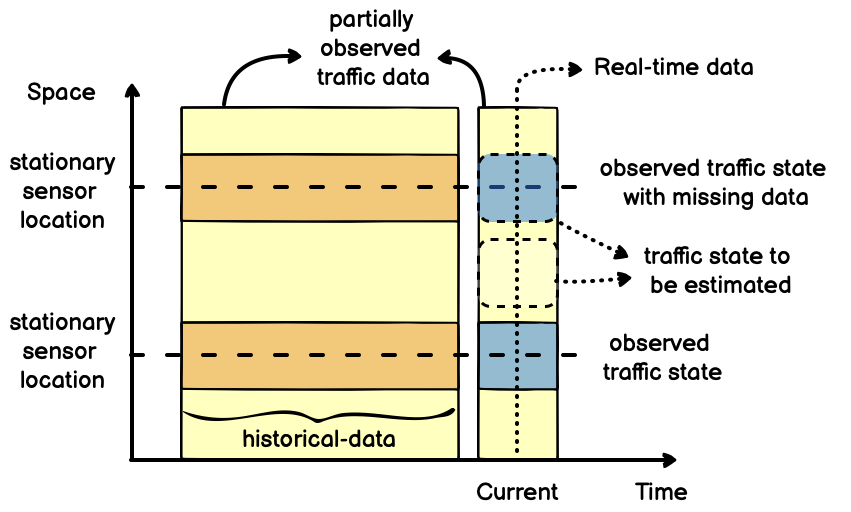
\includegraphics[width=0.8\textwidth]{tse_diagram.png}
    \caption{Relation of traffic data and traffic state in the space-time domain. Adapted from \cite{seo_tse}.}
    \label{fig:tse}
\end{figure}

Figure~\ref{fig:tse} is a conceptual diagram adapted from \cite{seo_tse}, which describes the traffic data, traffic state, and their relation in the time-space domain. Traffic state on highways can be represented by a subset of traffic variables, i.e., any two of three traffic state variables \cite{seo_tse}. In figure~\ref{fig:tse}, the traffic state is observable at the locations where stationary sensors are installed. However, stationary sensors are usually installed sparsely on highways due to cost reasons. In the regions outside stationary sensors' coverage, the yellow regions in figure~\ref{fig:tse}, traffic state variables are either unobserved or only partially observed through traffic data collected by other sensors, e.g., mobile devices. TSE aims to estimate the unobserved traffic state variables using partially observed traffic data in regions where stationary sensors are absent, e.g., the yellow region with the dashed boundary in figure~\ref{fig:tse} Besides, even at the locations where stationary sensors are installed, observed traffic data usually suffer from missing data points due to detector and communication malfunctions \cite{duan_dl_imputation, chen_imputation_regression}. Therefore, a type of TSE method called imputation is developed to estimate the missing data at locations where the traffic state is observed.

Data in figure~\ref{fig:tse} can be categorized into two groups according to the time when they are collected. If the data is collected when the traffic state is to be estimated, it is called real-time data or streaming data \cite{seo_tse}. Real-time data includes all kinds of traffic data collected by various sensors from the estimation location and its neighboring locations. On the other hand, if the traffic data is collected for a long time before the moment of estimation, it is called historical data, which also includes various types of traffic data collected from locations of interest. All TSE methods use real-time data and estimation models to infer traffic state variables, but not every TSE needs historical data. Historical data is utilized to calibrate and develop estimation models by some TSE approaches, e.g., model-driven and data-driven approaches.

Various traffic data measurements, e.g., stationary and mobile data, and various TSE approaches, e.g., model-driven, data-driven, and streaming-data-driven approaches, are used for estimating traffic state variables in the time-space regions of interest, which will be introduced in the later sections of this chapter. From now on, "time-space region/domain" and "spatiotemporal region/domain" will be used interchangeably.


\section{Traffic State Estimation Approaches}
\label{sec:tseApproaches}
According to the classifying method proposed by Seo et al. \cite{seo_tse}, TSE approaches can be grouped into three categories, i.e., model-driven, data-driven, and streaming-data-driven, depending on whether the approach needs a pre-determined assumption, i.e., a traffic flow model, and the data type they used. The approach adopted by this work belongs to the data-driven approach.

The \textbf{model-driven approach} uses pre-determined physical traffic flow models to estimate the traffic state \cite{seo_tse}. Those traffic flow models describing the dynamic of traffic were developed based on physical principles and empirical relations. They are well-formulated with a fixed model structure, e.g., functional forms, and a fixed number of parameters. The model parameters, i.e., the functions' parameters, are calibrated by historical data collected on the road segments/networks where the models will be implemented. The calibrated model will then estimate the traffic state in an unobserved region using real-time data as input. The model-driven approach is the most popular type of TSE approach that has been adopted by various studies in TSE, which could estimate traffic states accurately under ordinary traffic conditions \cite{seo_tse}.

The \textbf{data-driven approach} relies solely on historical data collected on the road without using physical models \cite{seo_tse}. It extracts the relationships between multivariate traffic variables from historical data, e.g., the dependence between the traffic state variable to be estimated and other observed variables, using statistical or ML methods. Similar to the model-driven approach, the data-driven approach uses the extracted dependence model to estimate the current traffic state based on real-time data. The same type of approach is also referred to as the "non-parametric approach" in the field of AI and traffic prediction \cite{van_traffic_prediction_models}, where machine learning models are extensively used. Non-parametric means both of the model structure, e.g., statistics functional form or ML algorithms, and the model parameters, i.e., functions' parameters or algorithms' parameters, are not determined in advanced but determined from the traffic data based on some evaluation metrics, e.g., RMSE and MAPE \cite{van_traffic_prediction_models}. Typically, a large amount of historical data is needed by data-driven approaches for building the dependence model. Recent ICT advances, e.g., IoT, have generated data increasingly from different sensor sources that are available for developing various data-driven approaches. Data-driven approaches, especially nonlinear ones such as neural networks, are good at modeling complex nonlinear relationships and traffic dynamics in the transportation field \cite{seo_tse, vlahogianni_forecast_overview, van_traffic_prediction_models}. Moreover, it does not need or need less prior knowledge on traffic to estimate the traffic state \cite{tsanakas_emission_estimation}. Generally speaking, the data-driven approach needs less domain-specific knowledge of the traffic process for estimation.

The \textbf{streaming-data-driven approach} uses only real-time data, i.e., streaming data, and some weak assumptions to estimate the traffic state in the unobserved region \cite{seo_tse}. Weak assumptions are some basic principles, e.g., conservation law in traffic flow theory, supported by physical theory and does not need empirical justification \cite{seo_tse}. Streaming-data-driven approaches do not need to extract dependence from historical data like data-driven approaches or calibrate the model parameters using historical data like model-driven approaches. However, it needs a large amount of streaming data to estimate the traffic state and usually has lower estimation accuracy than data-driven and model-driven approaches. On the other hand, because it does not rely on any empirical relations, it is more robust under uncertain phenomena and unpredictable conditions, e.g., traffic accidents \cite{seo_tse}.

\section{Fundamental Diagrams}
\label{sec:fd}
\gls{fd} are diagrams used in traffic flow theory to describe relations between traffic flow variables, i.e., flow, density, and speed, for a stationary traffic flow, where all vehicles have the same speed and spacing \cite{sumalee_future_ITS, Hoogendoorn_traffic_flow_theory_tu-delft}. Three diagrams in use are flow-density, flow-speed, and speed-density diagrams.

FD contains essential information on traffic characteristics such as free-flow speed, flow capacity, jam density, and the distinction between different traffic regimes, e.g., congested and free-flow regimes, essential for traffic control and traffic simulation \cite{dervisoglu_auto-calibrate_fd, seo_fd_probe}. Because FD describes the relations between traffic state variables, it is also utilized by both model-driven TSE \cite{seo_fd_probe} and data-driven TSE \cite{anuar_flow_probe} to estimate unobserved traffic state variables based on observed variables. Various mathematical functions have been proposed to describe empirical relations between traffic state variables in FDs using curve fitting techniques or traffic theories \cite{seo_tse, Hoogendoorn_traffic_flow_theory_tu-delft}. Figure~\ref{fig:triangular_fd} is an example of FD based on the popular triangular model proposed by Newell \cite{newell_triangular_fd}. 

\begin{figure}[!ht]
    \centering
    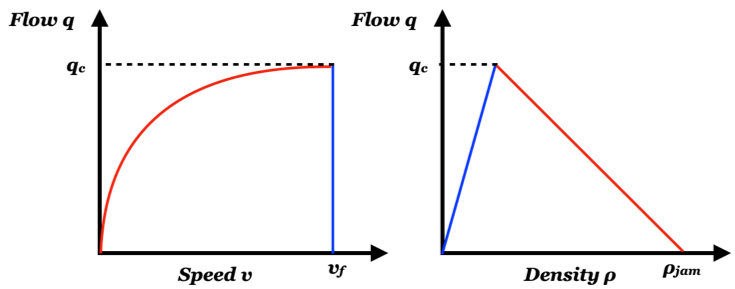
\includegraphics[width=\textwidth]{triangular_fd.png}
    \caption{Flow-speed and flow-density FD.}
    \label{fig:triangular_fd}
\end{figure}

In figure~\ref{fig:triangular_fd}, every point on the curve of the flow-speed relationship represents a specific traffic state characterized by flow and average speed. The density could be calculated based on flow and speed using equation \ref{eq:basic_traffic_variable_relation}. Some traffic state points in the FD provide us with essential information about highway facility traffic features. For the rightmost part of the flow-speed relation curve, i.e., the blue line, vehicles can travel at the maximum speed without inference from other vehicles in the traffic flow. The maximum speed is called free-flow velocity $v_f$, which depends on the operation's speed restrictions at a particular time and weather \cite{immers_traffic_theory_ku_leuven}. This traffic condition is called a free-flow regime, within which the density of vehicles is generally low. In the free-flow regime, the flow rate value can vary widely while the velocity remains constant. The maximum flow rate $q_c$ in the FD represents the road's capacity \cite{immers_traffic_theory_ku_leuven}. As the speed drops below $v_f$, the congestion begins, and the flow rate starts to decrease. The red curves in figure~\ref{fig:triangular_fd} represent the congested regime, where the speed and flow decrease while density increases. When the traffic is severely congested, flow and speed approach zero, and all vehicles are standstill. This traffic state is usually called traffic jam, and the density in this state is called jam density, $\rho_{jam}$.

Although the FDs were assumed to be invariant, the relation between traffic state variables in the real-world is not invariant but dynamic. The parameters of the relationship function and the function itself, i.e., the mathematical formula, vary depending on various factors. For example, many studies found that the empirical flow-speed relation observed at the same road segment varies on different days and in different traffic conditions \cite{neumann_bayesian, dervisoglu_auto-calibrate_fd, nguyen_online_calibration_fd_model}. The shapes of FD diagrams at different road segments collected from the same area could also be very different \cite{blandin_individual_speed}. Factors such as time, weather, road surface, accident, driver characteristics, and vehicles' composition can affect the shape of FDs \cite{seo_tse, Hoogendoorn_traffic_flow_theory_tu-delft}.

Many recent studies tried to capture the dynamic FD-relations using methods such as dynamically calibrating the model parameters or using ML clustering techniques to extract the relations \cite{neumann_bayesian, nguyen_online_calibration_fd_model, antoniou_ml_estimation}. The baseline model in this work is like a conventional static FDs used in many TSE studies \cite{anuar_flow_probe, blandin_individual_speed, neumann_static_fd_flow_estimation}, whose flow-speed relation does not change with time, space, and other factors. On the other hand, the \gls{ann} model proposed is more like a dynamic FD, which considers multiple factors, e.g., time, space, and other available features, that may affect traffic variables' relations.

\section{Machine Learning Methods}
\label{sec:ml}
This section aims to introduce machine leaning methods utilized in this work for extracting dynamic relations between traffic variables to empower our traffic flow estimator. Section~\ref{subsec:linearRegression} and \ref{subsec:polyRegression} introduce two simple machine learning models, linear regression and polynomial regression, which are used in our baseline model. Section~\ref{subsec:ann} introduces the deep neural network, an advanced machine learning method also known as deep learning. It is the main method used in this work to build the estimation model.

\subsection{Linear Regression}
\label{subsec:linearRegression}
Linear regression is one of the simplest machine learning techniques that have been widely used in both academic studies and industrial applications. Linear regression is a linear approach to model the relationship between a dependent variable, i.e., the value to predict, and independent variables, i.e., the feature values \cite{wiki_linearRegression, geron_handson_ml}. It assumes that the dependent variable is a linear combination of the parameters and the independent variables.

A typical linear regression model predicting a dependent variable based on multiple input features can be expressed as equation \ref{eq:linearRegression} \cite{geron_handson_ml}:

\begin{equation}
    \hat{y} = w_0 x_0 + w_1 x_1 + w_2 x_2 + \cdots + w_n x_n
    \label{eq:linearRegression}
\end{equation}

In equation~\ref{eq:linearRegression}, $\hat{y}$ is the predicted value, n is the number of features, and $x_i$ is the $i^{th}$ feature value. $w_j$ is the $j^{th}$ model parameter, which is the feature weight determining how much the $j^{th}$ feature affects the prediction. $w_0$ represents the bias term, i.e., intercept, while $x_0$ is always set to 1. Figure~\ref{fig:linearRegression} shows a training dataset and the predictions from a linear regression model with one dependent variable $x_1$. To be noticed that, it is typical to call the action of inferring dependent variables from features "prediction" in \gls{ml} field. Therefore, we use "predict/prediction" instead of "estimate/estimation" in this section to conform with the tradition.

\begin{figure}[!ht]
    \centering
    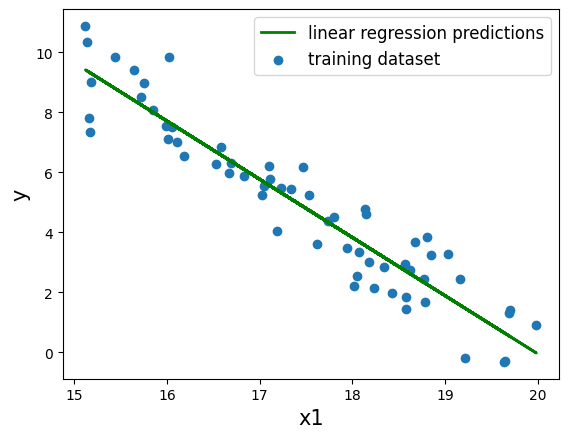
\includegraphics[width=0.7\textwidth]{linear_regression.png}
    \caption{Dataset with linear relationship and linear regression model predictions.}
    \label{fig:linearRegression}
\end{figure}

One crucial question is, how do we find the model parameters that best fit the training dataset? To solve the problem, we first need to define a cost function to measure the difference between the model’s predictions and the training examples. The most popular cost function used for the linear regression model is \gls{mse}, which is shown as equation~\ref{eq:costFunction} \cite{geron_handson_ml}:

\begin{equation}
J(\mathbf{w})=MSE(\mathbf{w})=\frac{1}{m}\sum_{i}^{m}(\hat{y}^{i}-y^{i})^{2}
\label{eq:costFunction}
\end{equation}

In equation~\ref{eq:costFunction}, $\mathbf{w}$ is the parameter vector, and $m$ is the number of samples in the training dataset. $y^i$ is the dependent variable's value of $i^th$ sample, while $\hat{y}^{i}$ is the corresponding predicted value by the linear regression model. $J(\mathbf{w})$ is defined as the MSE of the model, which measures how close the predicted values to the real values under a particular value of $w$. The goal of learning is to choose model parameters that minimize the cost function so that the prediction values are closest to the values in the training dataset.

Two popular approaches are utilized by machine learning software frameworks to find model parameters, the Normal Equation and the Gradient Descent \cite{geron_handson_ml}. For the first approach, one directly solves the normal equation, where the gradient of cost function equals 0, to obtain the parameter vector $w$ that minimizes the cost function \cite{geron_handson_ml}. However, the computational complexity for solving the normal equation is $O(n^3)$, which make this approach very slow while the number of features in equation~\ref{eq:linearRegression} grows large. Another approach is gradient descent, which finds the optimal solution of model parameters that minimize the cost function by changing the parameters iteratively \cite{geron_handson_ml}. The algorithm of gradient descent starts from a parameter vector w with random values, then iteratively changes the parameters toward the direction of the descending gradient until the cost function converges to the minimum value. This optimization algorithm is more computationally efficient than solving the normal equation when the number of features is large. Gradient descent not only can be used to find the optimal solution for linear regression, but it is also the core algorithm for training neural networks, which will be introduced in section~\ref{subsec:ann}.

Many TSE and traffic forecasting studies used linear regression as their prediction model or as a baseline model to compare with more sophisticated models \cite{blandin_individual_speed, chen_imputation_regression, nikovski_univariate_prediction}. Its simplicity and computational efficiency give it a competitive edge while memory constraint and short execution time, e.g., real-time application, are critical requirements.

\subsection{Polynomial Regression}
\label{subsec:polyRegression}
Polynomial regression is a technique that uses the linear model to fit the nonlinear relationships \cite{geron_handson_ml}. It adds the power of the independent variables $x$ in equation~\ref{eq:linearRegression} as new features to model the nonlinear relationship between $x$ and the predicted value $\hat{y}$. For example, a univariate nth degree polynomial regression model can be expressed as equation~\ref{eq:polynomialRegression}:
\begin{equation}
    \hat{y} = w_0 x_0 + w_1 x + w_2 x^2 + w_3 x^3 + \cdots + w_n x^n
    \label{eq:polynomialRegression}
\end{equation}

Although one could use polynomial regression to fit nonlinear relationships between variables, polynomial regression is considered to be a kind of linear regression since the predicted value is still a linear combination of parameters and independent variables. One should avoid overfitting when using high-degree polynomial regression to fit the data by using techniques such as cross-validation. Some studies of FD used polynomial regression as the model to fit the nonlinear relationships between traffic state variables \cite{nguyen_online_calibration_fd_model}.

\subsection{Artificial Neural Network}
\label{subsec:ann}
The artificial neural network, or just the neural network, is originally a computational model inspired by the biological neural networks proposed by McCulloch \cite{mcculloch_ann_origin}. As the subject evolved, many improvements in model structures, e.g., \gls{mlp} \cite{rosenblatt_mlp}, and algorithms for training multi-layer neural networks, e.g., backpropagation algorithm, were proposed \cite{rumelhart_back_propagation}, which form the deep neural networks we are using nowadays. Following the increasing computational power because of the exponential increment of transistor number in microprocessors, more practical neural networks can be deployed by the computers after the 1980s.

\begin{figure}[!ht]
    \centering
    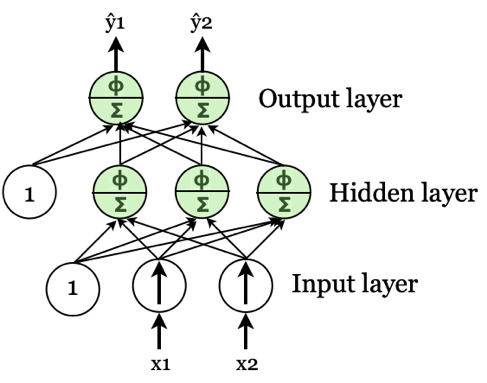
\includegraphics{ann_conceptual_diagram.png}
    \caption{Architecture of a neural network with one input layer, one hidden layer, and one output layer. Adapted from \cite{geron_handson_ml}.}
    \label{fig:annConceptual}
\end{figure}

Figure~\ref{fig:annConceptual} shows the architecture of a neural network with one input layer, one hidden layer, and one output layer. The structure is also called MLP or deep neural network because it has more than one layer of perceptron in the model. The input layer includes the input feature variables of the model plus a bias input which always equals one. Each green node in the figure is an artificial neuron, which emulates the biological neuron. Each neuron has several input neurons as well as a bias input. Each input connection has its corresponding weight. The neuron computes the weighted sum of all inputs, then apply an activation function to the weighted sum, whose output value will be the output of the neuron. There is a wide range of choices for the activation function, e.g., sigmoid, tanh, and ReLu \cite{geron_handson_ml}, which should be chosen carefully considering functions' performance and the type of prediction problem to solve. The outputs of neurons in a layer will be the input for neurons in the next layer. The last layer's outputs, i.e., the outputs of the output layer, are the predicted values of the whole neural network. As the signal can only flow in one direction from the input layer, through hidden layers, to the output layer, this architecture is also called feed-forward neural network. The outputs of a whole neuron layer can be computed with equation~\ref{eq:perceptronLayerOutput} \cite{geron_handson_ml}:

\begin{equation}
    h_{\mathbf{W},\mathbf{b}}(\mathbf{X})=\phi(\mathbf{XW}+\boldsymbol{\mathbf{b}})
    \label{eq:perceptronLayerOutput}
\end{equation}

In equation~\ref{eq:perceptronLayerOutput}, $\mathbf{X}$ is the matrix of input features or input neurons. Each row represents an instance, and each column represents an input feature/neuron. $\mathbf{W}$ is the weight matrix contains all connection weights for inputs except the weights for the bias input. $\mathbf{b}$ is the bias vector contains the weights for the bias input, which has one weight value for each neuron in the layer. $\mathbf{W}$ and $\mathbf{b}$ are model parameters of the neural network, which should be initialized randomly and learned from the training data. $\phi$ represents the activation function of the neurons. For hidden layers, it is usually a nonlinear function in order to add nonlinearity to the neural networks. For output layers, the choice of activation function dependents on the type of prediction problem, e.g., sigmoid is usually used for binomial classification. In contrast, a simple linear function is used for regression problems.

To learn neural network's model parameters, i.e., $\mathbf{W}$ and $\mathbf{b}$ in equation~\ref{eq:perceptronLayerOutput}, and minimize the error of predictions, we first need a cost function similar as the one for linear regression that measures the error between the predicted values and the training data. For regression problems, we use MSE as the cost function for neural networks, which is the same cost function we used in linear regression. For classification problems, cross-entropy is the cost function that is widely used. The algorithm that is widely used for training neural networks is called backpropagation training algorithm \cite{rumelhart_back_propagation}. Backpropagation algorithm used two steps and gradient descent repeatedly to minimize cost function's value \cite{geron_handson_ml}. In the first step, the algorithm computes the prediction and measures the prediction error by feeding the input features forwardly from the input layer to the output layer, which is called the forward pass. In the second step, the algorithm goes in reverse from output error to the input layer to compute the gradients of cost function corresponding to every connection weight, which is called the backward pass. Finally, the gradients computed will be used in the gradient descent, which was mentioned in section~\ref{subsec:linearRegression}, to change weights of neural networks to reduce cost function's value.

Neural networks are non-parametric machine learning models that are powerful to learn highly nonlinear relationships in high-dimensional data \cite{vlahogianni_forecast_overview, ma_lstm_predict}, which is suitable to model complex relationships lying in transportation datasets. Because of their advantages and ability to make accurate predictions, neural networks are widely used in scientific and industrial applications, e.g., computer vision, natural language processing, and transportation applications such as traffic forecasting.

\section{Related Works}
\label{sec:relatedWorks}
Previous studies using data-driven approaches for estimating traffic state variables from mobile data mainly focused on extracting the relationships between traffic flow and other traffic variables lying in stationary historical data by using statistical or machine learning models. After the relation model is built, streaming mobile data is used as input to estimate the traffic flow or other traffic variables. Blandin et al. \cite{blandin_individual_speed} and Bulteau et al. \cite{Bulteau_flow_higher-order} used linear regression to fit FD-like relations between traffic flow and speed/speed variance in un-congested states. Wilby et al. \cite{wilby_flow_estimation_xfcd} also proposed a method that utilized linear regression to model the relations between flow and traffic variables collected from extended floating car data for different traffic regimes, e.g., free-flow and congested traffic. However, the approaches proposed by these works require either manually identification or computationally complex algorithms to determine the segmentation thresholds between different traffic conditions/regimes, which are not scalable traffic estimation solutions. The linear models are also not suitable for multivariate modelling, which incorporates multiple dependent variables for estimation and should benefit from the increasing data sources emerging from the Internet of Things. Anuar et al. \cite{anuar_flow_probe} used multiple FD functions from traffic flow theory to fit the flow-speed relationships in a stationary dataset. The authors then derived the traffic flow from mobile data speed and compared the estimation accuracy corresponding to each fitted model. The model proposed by this work is more restrictive to the functional forms that were chosen by authors for fitting the flow-speed relationship than other data-driven approaches. TSE approaches mentioned above used stationary relationships between two traffic variables for estimation, which cannot capture the temporal or spatial dependency of dynamic relationships mentioned in section~\ref{sec:fd} .

Some studies tried to model the dynamic relationships between traffic variables when developing their estimation models. Neumann et al. \cite{neumann_bayesian} proposed a stochastic approach to model the dynamic flow-speed relationship by using Bayesian networks and used the models to estimate the traffic flow from mobile data, speed, in a wide area. The approach considered the temporal dependencies and transitions between traffic states when extracting the relationship from the historical dataset. Antoniou et al. \cite{antoniou_ml_estimation} proposed a non-parametric ML-based approach that incorporated multiple traffic variables for estimating speed. Although this approach was not developed for estimating flow but for estimating speed from density and flow, it could also be used for flow estimation from traffic variables collected from mobile sensors. The proposed estimation approach used a combination of several ML methods, including k-means clustering, locally weighted regression, and \gls{knn} classification. It also can capture the dynamic relationship between traffic variables and the change in traffic conditions. The study is also one of few studies, to the best of author's knowledge, that used multiple traffic data as dependent variables, i.e., input features, for estimating the traffic state. However, the ML methods used in this work are not suitable for modelling datasets with high dimension, i.e., the number of feature variables, and large size, i.e., the number of instances in the dataset. For example, k-means clustering and KNN classification both suffering from the "Curse of Dimensionality", which means they do not perform well in high-dimensional data. k-nearest-neighbor also needs long computational time to classify an instance when the size of the training dataset is large because the computational complexity of KNN is proportional to the number of instances in the dataset. Besides, some model-driven TSE approaches were developed to capture the time-varying relationships by updating the model parameters dynamically, i.e., on-line calibration \cite{nguyen_online_calibration_fd_model, wang_tse_online_calibration}.

Compared with previous works of data-driven TSE using mobile data, the approach proposed in this work is highly automated and simple to implement with no need for human intervention in model building. The proposed neural network model captures not only temporal but also spatial dependencies of the relationship between traffic variables to make an accurate estimation in a wider time-space region on the highway. Besides, thanks to the neural network's ability of modelling complex nonlinear relationships between data variables in large datasets with a multivariate setting, the proposed approach is flexible to incorporate various available information, e.g., travel time, as input features in addition to the classic traffic state variables for estimation.

\chapter{Datasets and Methodology}
\label{ch:methodologyAndDatasets}
This chapter provides an overview of the datasets and the methods used in the thesis project. We first describe the two traffic datasets on which the project is built. The remaining sections then present the processes and techniques we adopted during the project's implementation, including data preparation, model training, and evaluation metrics.

\section{Datasets}
\label{sec:datasets}
Traffic data provided by two sensor platforms are used to train and test the estimation models in the thesis, i.e., the INRIX and the \gls{mcs}. INRIX datasets belong to the mobile data, while MCS datasets are a kind of stationary data introduced in section~\ref{sec:dataTypes} The data are collected from two consecutive road segments on the four-lane E4 highway, southbound, in Stockholm from 2018-10-01 to 2018-10-31. Figure~\ref{fig:inrixMcsLocation} shows the locations of INRIX road segments and MCS sensors on the map. Table~\ref{tab:segmentIDs} lists the IDs for INRIX road segments and MCS sensors in the datasets. We use "south" to denote segment 1071883675 and sensor 1159 and use "north" to denote segment 225285973 and sensor 1162 in the thesis.

\begin{figure}[!ht]
    \centering
    \begin{subfigure}{0.49\textwidth}
        \centering
        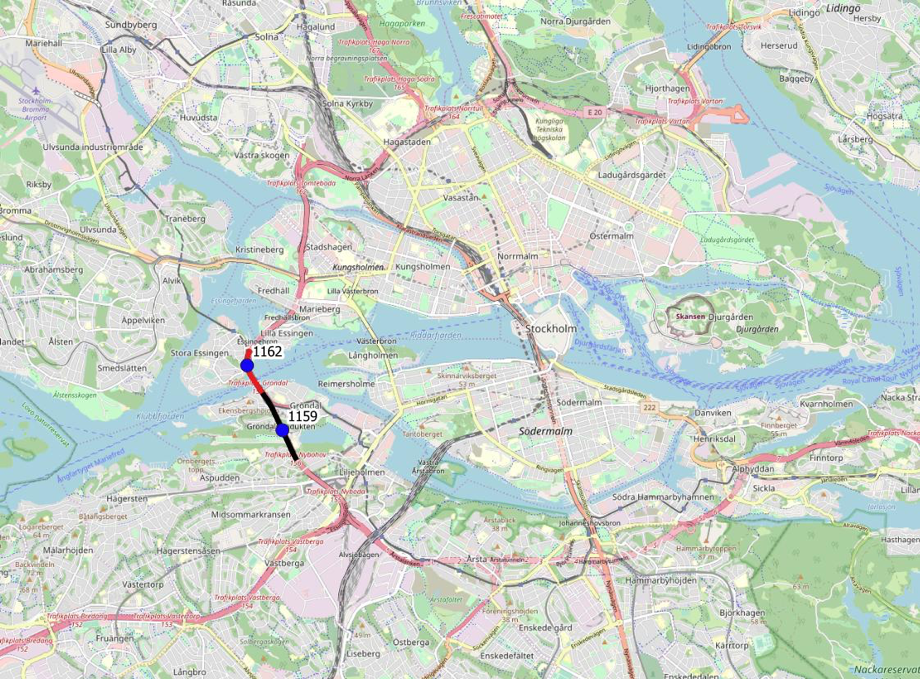
\includegraphics[width=\textwidth]{inrix_mcs_location_a.png}
        \caption{Sensor's locations in Stockholm}
    \end{subfigure}
    \hfill
    \begin{subfigure}{0.49\textwidth}
        \centering
        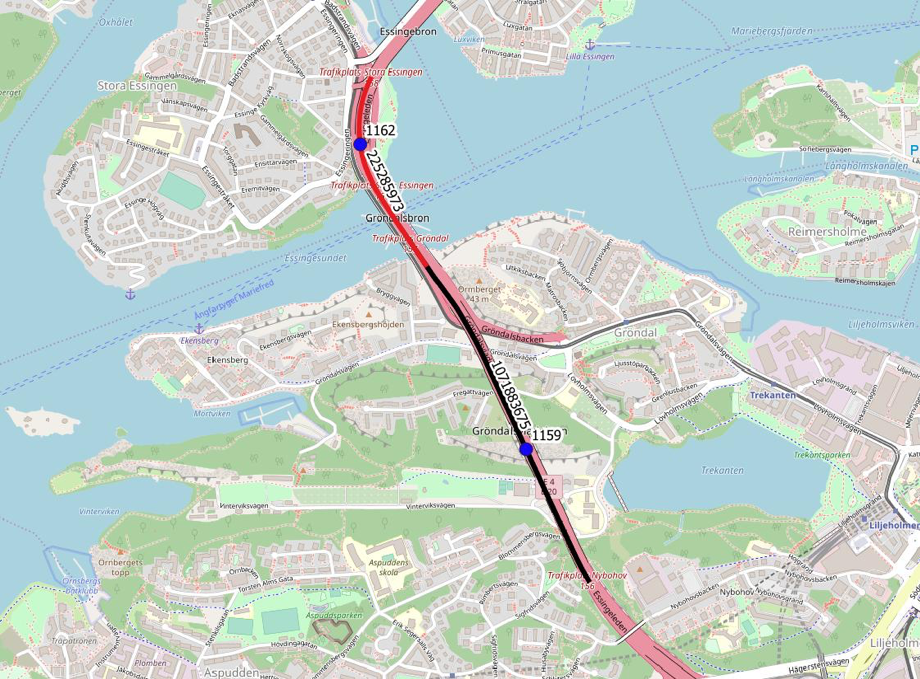
\includegraphics[width=\textwidth]{inrix_mcs_location_b.png}
        \caption{Enlarged geographical map}
    \end{subfigure}
    \caption{Locations of INRIX segments and MCS sensors in Stockholm.}
    \label{fig:inrixMcsLocation}
\end{figure}

\begin{table}[!ht]
\centering
\begin{tabular}{@{}lll@{}}
\toprule
\textbf{Road Segment} & \textbf{INRIX ID} & \textbf{MCS ID} \\
\midrule
South          & 1071883675 & 1159     \\
North          & 225285973  & 1162     \\ 
\bottomrule
\end{tabular}
\caption{INRIX ID and MCS ID for corresponding road segments.}
\label{tab:segmentIDs}
\end{table}

The first three weeks of data, i.e., 1\textsuperscript{st} to 21\textsuperscript{st} October, are used as training datasets for building/training each estimation model, and the following one week of data, i.e., 22\textsuperscript{nd} to 29\textsuperscript{th} October, from both road segments are used as test datasets for evaluating the application of the models. Both platforms provide aggregated traffic measurements, timestamps, and other traffic-related information at a frequency of once every minute, and both data are delivered in \gls{csv} format. Detailed information about two data sources and the traffic information they provide is presented in the following sections.

\subsection{INRIX}
\label{subsec:inrix}
INRIX combines data from many sources to provide traffic information. A major part of the data comes from a crowdsourced model where INRIX continuously collects speed and location from probe vehicles, combines the data into an updated view of the current traffic situation on the road, and sends it back to the vehicles. In a press release in May 2010\footnote{"INRIX’s Crowd-Sourced Traffic Network Surpasses 2 Million Vehicles", INRIX press release, May 5, 2010. <https://inrix.com/press-releases/2650/>, viewed 5 June 2020.}, INRIX said they had a network of two million GPS-enabled vehicles: \textit{“Providing a foundation of continuous real-time speed and location reports to INRIX every minute for an average of 7 hours per day, per vehicle, commercial fleets – such as taxi cabs, service delivery vans and long haul trucks – represent the majority of INRIX’s network. INRIX intelligently combines these reports with data from consumer vehicles and GPS-enabled smartphones to deliver a service that updates traffic information to drivers every minute, ensuring they have the most accurate view of traffic conditions wherever they go.”}

Table~\ref{tab:inrix_schema} shows the schema and an example of data from the INRIX dataset. Data fields in bold in table~\ref{tab:inrix_schema} are the variables of interest in the project.

\begin{table}[!ht]
    \begin{tabular}{@{} m{0.15\textwidth} m{0.64\textwidth} m{0.16\textwidth} @{}}
    \toprule
    \textbf{Field} & \textbf{Description} & \textbf{Example} \\
    \midrule
    \textbf{Segment ID} & An identifier for defining a unique road segment. & \textbf{1071883675} \\ 
    \midrule
    \textbf{Timestamp} & The timestamp of the measurement in UTC. & \textbf{2018-10-01 00:00:12} \\
    \midrule
    Segment Type & Type of road segment: XD Segment (XDS) or TMC segment. & XDS \\
    \midrule
    \textbf{Speed} & Average speed of vehicles on the segment calculated from the most current time slice, in km/h. & \textbf{93} \\ 
    \midrule
    Average Speed & The historical average speed on the segment for the given day and time (km/h). & 68 \\ 
    \midrule
    Reference Speed & An expected free-flow speed on the segment, determined from the INRIX traffic archive (km/h). & 68 \\ 
    \midrule
    \textbf{Travel Time} & The time required to travel across the segment in minutes. & \textbf{0.738} \\ 
    \midrule
    \textbf{Score} & A measure of confidence in a given reported speed with three possible values: 10/20/30 \cite{kim_inrix_data_comparing}. Samples with confidence score larger than 10 are based on real-time data, otherwise are based on historical data. & \textbf{30} \\ 
    \midrule
    Cvalue & The second measure of confidence ranges from 0 to 100, which only applies when the confidence score is 30 \cite{kim_inrix_data_comparing}. & 49 \\ 
    \midrule
    Speed-bucket & Level of congestion according to the range of speed. & 3 \\
    \bottomrule
    \end{tabular}
    \caption{The schema and example of the INRIX dataset}
    \label{tab:inrix_schema}
\end{table}

To be noticed that the speed reported by INRIX every minute is space-mean speed calculated from the most current time slice \cite{sharma_inrix_data_opportunity}. In the thesis project, speed and/or travel time are used as main input features for estimation models. In contrast, timestamp and segment ID are used for preparing temporal and spatial factors in the feature vector for capturing time and space dependency of the traffic relationship.


\subsection{Motorway Control System (MCS)}
\label{subsec:mcs}
The traffic flow in Stockholm is monitored with the \acrfull{mcs} by the Swedish transport administration (Trafikverket). Many stationary MCS-portals have been installed on the gantries on the E4 highway and other roads in Stockholm's road network. The MCS-portals are equipped with radar sensors, which monitor the traffic flow and speed in each lane of the road every minute. The data provides the regional traffic control center with information about the current traffic flow and speeds. The data is also input to a control system that sets variable speed limit signs.

\begin{table}[!h]
\begin{tabular}{@{}m{0.15\textwidth} m{0.6\textwidth} m{0.2\textwidth}@{}}
\toprule
\textbf{Field} & \textbf{Description} & \textbf{Example} \\
\midrule
Fk\_id & Reference ID identifying the location of sensor on the road. & 1159 \\ 
\midrule
Timestamp & The timestamp of the measurement. & 2018-10-01 00:01:00 \\ 
\midrule
\textbf{Speed} & Average speed of vehicles passing the sensors in the past minute, in km/h. & \textbf{93.816} \\ 
\midrule
\textbf{Flow} & Flow rate in veh/h, calculated from the   number of vehicles passing the sensors in the past minute. & \textbf{160} \\ \midrule
Used Lane & The lanes contribute to the measurements in the past minutes. NULL indicates there are no vehicles on the lane. & 1,1,1,NULL \\ 
\bottomrule
\end{tabular}
    \caption{The schema and example of the MCS dataset}
    \label{tab:mcs_schema}
\end{table}

The distance between the locations of two MCS sensors in this work is 1 km. The MCS measurements are aggregated over a minute while reported by the system. MCS measurements are fixed-point measurements and hence provide time-mean speed as reported speed after aggregation. On the other hand, the probe measurements such as INRIX calculate the space-mean speed over a road segment as vehicles' reported average speed  \cite{sharma_inrix_data_opportunity}. Different measurement techniques also lead to bias and delay in INRIX data compared to stationary sensor speed \cite{sharma_inrix_data_opportunity, kim_inrix_data_comparing}. To be noticed that the MCS datasets used in this project have been further aggregated over raw sensor data from all lanes on E4 to obtain average flow and speed on the road.

The schema of the MCS datasets and an example from the south segment are shown in table~\ref{tab:mcs_schema}. Data fields in bold are the variables selected and used in the project. The traffic flow in MCS datasets is used as labels for training and testing the project's estimation models. On the other hand, we use MCS speed data as a benchmarked speed for mitigating the latency exhibited by the INRIX data during the data preparation.

\section{Data Preparation}
\label{sec:dataPreparation}
Various data exploration and preparation techniques are adopted to prepare the datasets, including feature vectors and labels, to train and test the estimation models. Techniques such as plotting and statistical measures, e.g., correlation coefficient, are used in the explorative analysis to get insights into the datasets and evaluate the effect of data preparation on the variables. Regarding data preparation, the following techniques of feature engineering for machine learning are adopted for preparing the datasets:

\begin{itemize}
    \item Filtering: The INRIX datasets contain data points with a low confidence score (10), which always report the same speed value equals the historical reference speed, and thus cannot reflect the real-time traffic condition on the road segment. We filter out these data points in INRIX datasets to ensure the traffic variable values represent the traffic condition at the moment of measuring.
    \item Smoothing: The measurements of traffic variables, i.e., flow, speed, are noisy in INRIX and MCS datasets. We need to remove noise and expose the variable values that signify the real trends to increase the models' estimation accuracy. Moving average with a window width of 30 time-steps is adopted for smoothing the speed, flow, and travel time.
    \item Shifting: A 6-minute latency of speed is observed in INRIX datasets compared with the MCS speed. This lag-time is within the latency range, from 6 to 8 min, reported by various studies \cite{kim_inrix_data_comparing}. We eliminate the latency by shifting the INRIX time-series by 360 s to ensure the measurements from both types of datasets reflect the same traffic condition in the same timestamp. Besides, INRIX and MCS's timestamps were registered in different time-zones, requiring time-series shifting to match the timestamps from two platforms beforehand.
    \item One-hot Encoding: One-hot encoding \cite{geron_handson_ml} is adopted to convert INRIX's timestamps and segment IDs into time-related features and space-related with a numerical form for ANN models. We prepare two time-related features and one space-related feature to help estimation model extracting time and space-dependent traffic relationships:
    
    \textbf{hour feature}: the hour "part" in the timestamp is converted into a 24-bit one-hot code, which represents the hour of observation in a day.
    
    \textbf{day feature}: the "day" part in the timestamp is converted into a 2-bit one-hot code, representing the day of observation in a week, i.e., on weekdays or weekends.
    
    \textbf{location feature}: the "segment ID" is converted into a 2-bit one-hot code, representing the location of the observation on the E4, i.e., on the south or north segment.
    
    Table~\ref{tab:oneHot} shows an example of one-hot encoding time and space features for an INRIX data point measured at 20:00 Wednesday on the south segment, together with its original timestamp and segment ID.

\begin{table}[]
\begin{tabular}{@{} m{0.15\textwidth} m{0.3\textwidth} m{0.5\textwidth}@{}}
\toprule
\multicolumn{2}{l}{Timestamp, Segment ID} & 2018-10-03 20:21:00, 1071883675 \\ 
\midrule
\multirow{3}{4em}{One-hot Encoding} & hour feature {[}00, 01, …, 23{]} & {[}0, 0, 0, 0, 0, 0, 0, 0, 0, 0, 0, 0, 0, 0, 0, 0, 0, 0, 0, 0, 1, 0, 0, 0{]} \\ 
\cmidrule(l){2-3} 
& day feature {[}weekday, weekend{]} & {[}1, 0{]} \\ 
\cmidrule(l){2-3} 
& location feature {[}south, north{]} & {[}1, 0{]} \\ 
\bottomrule
\end{tabular}
\caption{Example of one-hot encoding features for temporal and spatial factors.}
\label{tab:oneHot}
\end{table}
    
    \item Feature Scaling: A machine learning model's input attributes need to be on the same scale for the machine learning algorithm to perform well. Two methods are commonly used to scale the input attributes, i.e., normalization and standardization. We adopt standardization to scale the numerical attributes for neural networks, i.e., speed and travel time, because it is less affected by the outliers in datasets than the normalization. Standardization first subtracts the mean value of the dataset from the feature values, then divides them by the standard deviation, as shown in equation~\ref{eq:standardization}. The standardized input attribute has a zero mean and a unit deviation in its distribution.
    
    \begin{equation}
        {x}'=\frac{x-\bar{x}}{\sigma}
        \label{eq:standardization}
    \end{equation}
    \begin{align*}
    & {x}'=the \ standardized \ input \ feature \quad x=the \ original \ feature \\
    & \bar{x} = the \ mean \ of \ the \ feature \ values\\
    & \sigma = the \ standard \ deviation \ of \ the \ feature \ values
    \end{align*}
\end{itemize}

\section{Model Training}
\label{sec:modelTraining}
Our goal is to develop an approach that automatically finds relationships between observed variables in INRIX data and the flow in MCS data, which can later be used for estimating un-observed flow from the INRIX data collected in the future and the neighboring area. These relationships are the flow estimation models which we are going to train and test using prepared datasets. Two types of models are trained in this work: a multi-regime baseline model and ANN models. The multi-regime baseline model acts as a benchmark for comparison with the ANN models proposed, while ANN models are built for the purposes listed in section~\ref{sec:goalAndPurposes}. Two types of models are trained in this work: a multi-regime baseline model and ANN models.

\subsection{Baseline Model}
\label{subsec:baselineModel}
Multi-regime models are widely used for modeling the relationships of traffic variables \cite{tsanakas_emission_estimation, blandin_individual_speed, antoniou_ml_estimation, nielsen_flow-speed_relations}, which use different functional forms for modeling the relationships in different traffic regimes in FDs, e.g., free-flow and congested regime. Univariate linear regression is often used to characterize the linear relationships between flow and speed in the free-flow regime \cite{blandin_individual_speed, nielsen_flow-speed_relations}. For the congested regime, curved relationships between flow and speed are often observed, and the functional form derived from the linear relationship between flow and density is often used to characterize the relationship \cite{blandin_individual_speed, nielsen_flow-speed_relations}.

\begin{equation}
    \hat{q} = 
    \left \{\begin{matrix}
    av + b & if \ v > v_c\\ 
    cv^2 + dv + e & otherwise
    \end{matrix}\right.
    \label{eq:baseline}
\end{equation}
\begin{align*}
    & \hat{q} = estimated flow \quad v = speed \quad v_c=critical \ speed \\
    & a,b,c,d,e=model \ parameters
\end{align*}

We train a multi-regime model on the training dataset of south segment as our baseline model for later comparison with more sophisticated ANN models. The mathematical expression for the baseline model is shown in equation~\ref{eq:baseline}. All sample speeds higher than or equal to the critical speed, 70km, are categorized as free-flow and are regressed onto flows using linear regression. The samples with speed lower than the critical speed are categorized into the congested regime, and their flow is modeled as a second-degree polynomial in speed. The critical speed is manually determined from the flow-density diagram. The density is derived from the MCS flow and INRIX speed using the traffic variable relation in equation~\ref{eq:basic_traffic_variable_relation} \cite{blandin_individual_speed, nielsen_flow-speed_relations}. The degree of the polynomial regression is determined by the hyperparameter tuning using 10-fold cross-validation.

\subsection{Neural Network Models}
The project aims to develop model structures that produce accurate flow estimation results from INRIX data by utilizing the neural network's ability to learn and model high-dimensional and non-linear relationships. We construct five neural network models to evaluate the neural network's performance in modeling classic flow-speed relationship, the relationship between traffic flow and multiple input features, and time-space-dependent relationships using prepared datasets.

\begin{figure}[!ht]
    \centering
    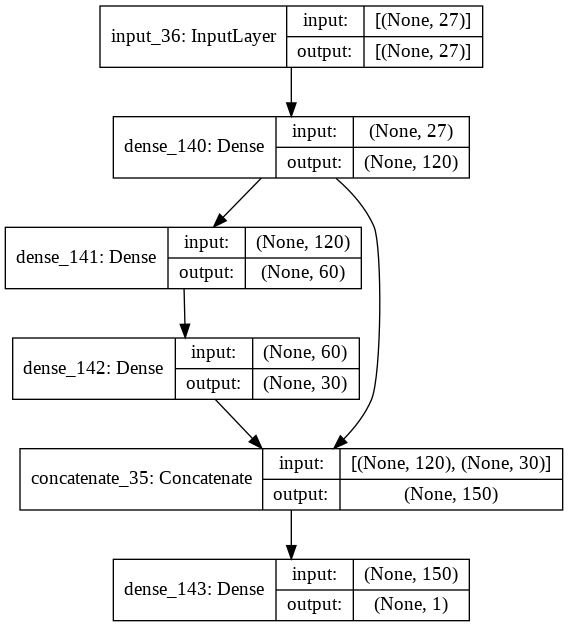
\includegraphics[width=0.65\textwidth]{temporal_ann_structure.png}
    \caption{Structure of the neural network considering temporal dependencies.}
    \label{fig:temporal_ann_structure}
\end{figure}

All proposed neural networks are based on an architecture called "Wide \& Deep Learning," introduced in a 2016 paper \cite{cheng_w&d_learning}. The architecture enables ANN to learn both deep patterns through deep neural network layers and simple patterns in data by connecting the inputs directly to the output layer \cite{geron_handson_ml, cheng_w&d_learning}. Each neural network consists of six layers: one input layer, three hidden layers, one concatenate layer and one output layer. The first layer is an input layer with dimension n equals to the number of input features. For example, if the model's independent variables are speed and travel time, n equals two. The input layer is followed by three densely connected hidden layers containing 120, 60, and 30 neuron nodes, respectively. The number of neuron units in each hidden layer is determined by hyperparameter tuning. The first and third dense hidden layer outputs are fed into a concatenate layer, which merges the outputs of two layers and feeds the concatenation to the output layer. The purpose of the concatenate layer is to provide a short path to the model, through which it can learn simple and undistorted patterns from the layer closer to the input features. The last layer of the model is an output layer, which densely connects its inputs and produces a predicted value of traffic flow on the road segment as the entire estimator's output. The dimension of the output layer is one for all neural network models. Figure~\ref{fig:temporal_ann_structure} shows the structure of one of the proposed ANN models with 27 input features, including speed, hour, and day features, which are listed in table~\ref{tab:oneHot}.

"None" in input and output shapes in figure~\ref{fig:temporal_ann_structure} means the number of samples in the data batch is not fixed but flexible for different datasets. We use MSE as the cost function and Adam algorithm, an extension of gradient descent algorithm, as our optimization algorithm for training the neural networks. More details about each neural network and its corresponding purpose are presented as follows.

\subsubsection{Univariate Neural Network}
\label{subsubsec:univariateNeuralNetwork}
The ANN model characterizes the simple flow-speed relation with a single independent variable, speed. The mathematical representation of the estimation model is shown as equation~\ref{eq:ann_spd}.


The purpose of this univariate neural network is to evaluate ANN's ability to learn and model the stationary flow-speed relationship from the data compared with the traditional baseline model. The model is trained on the INRIX speed and MCS flow in training datasets collected from the south road segment from 1\textsuperscript{st} to 21\textsuperscript{st} October. In order to evaluate the model's estimation accuracy and its generality for the adjacent road segment, we test the model on the test datasets, as mentioned in section~\ref{sec:datasets}, collected from both the south and north segments in the following week.

\begin{equation}
    \hat{q} = E(v)
    \label{eq:ann_spd}
\end{equation}
\begin{align*}
    & \hat{q} = estimated \ flow \quad v=speed
\end{align*}

\subsubsection{Multivariate Neural Network}
\label{subsubsec:multivariateNeuralNetwork}
We incorporate travel time, another real-time information of road traffic provided by INRIX, as an additional feature for flow estimation. The multivariate neural network with two input features, speed and travel time, is constructed to evaluate ANN's ability to capture non-linear relationships between multiple traffic variables, which is a more complicated task when only using linear regression. Moreover, the model is used to evaluate whether the travel time is a useful feature that can provide additional information than speed to improve the estimation accuracy. 

\begin{equation}
    \hat{q} = E(v,tt)
    \label{eq:ann_spd_tt}
\end{equation}
\begin{align*}
    & \hat{q} = estimated \ flow \quad v=speed \quad tt = travel \ time
\end{align*}

\subsubsection{Neural Network with Temporal Dependency}
\label{subsubsec:temporalNeuralNetwork}
A neural network that considers the temporal dependency of the flow-speed relationship is constructed. The neural network incorporates time-related features, i.e., hour and day features introduced in section~\ref{sec:dataPreparation}, as its inputs to capture the dynamic flow-speed relationship, which changes with different hours in a day and different days in a week. The structure of this neural network was already shown in figure~\ref{fig:temporal_ann_structure}, and the mathematical representation of the model is shown as equation~\ref{eq:temporal_ann_spd}. To be noticed that the hour feature is a 24-bit one-hot encoding representing each hour in a day, and the day feature is a 2-bit one-hot encoding representing weekday or weekend. Therefore, the model has an input vector with a dimension of 27. The model is also trained on south segment data and tested on data from both road segments in the following week.
\begin{equation}
    \hat{q} = E(v,h,d)
    \label{eq:temporal_ann_spd}
\end{equation}
\begin{align*}
    & \hat{q} = estimated \ flow \quad v=speed \quad h=hour \ in \ a \ day \\ & d=day \ in \ a \ week \ (weekday \ or \ weekend)
\end{align*}

\subsubsection{Multivariate Neural Network with Temporal Dependency}
\label{subsubsec:temporalMultivariateNeuralNetwork}
Like the multivariate ANN, this neural network incorporates travel time in addition to the speed as the second input feature. The difference is that this ANN also considers the temporal dependency of traffic conditions by incorporating the time features, i.e., hour and day.

The purpose of this model is to examine whether the travel time as an additional independent variable can improve the estimation accuracy when the model also captures the transitions of the traffic conditions over time.
\begin{equation}
    \hat{q} = E(v, tt, h,d)
    \label{eq:temporal_ann_spd_tt}
\end{equation}
\begin{align*}
    & \hat{q} = estimated \ flow \quad v=speed \quad  tt=travel time \\
    & h=hour \ in \ a \ day \quad d=day \ in \ a \ week \ (weekday \ or \ weekend)
\end{align*}

\subsubsection{Neural Network with Spatiotemporal Dependency}
\label{subsubsec:spatiotemporalNeuralNetwork}
Finally, we construct a neural network considering both temporal and spatial dependencies when modeling the flow-speed relationship. The model is trained on data from both road segments, i.e., south and north, with time-related input features, i.e., hour and day, and a 2-bit location feature that identifies the road segments. Same as other models, the model is tested on the data collected from both road segments in the following week.
In general, the flow-speed relationship varies with time and locations in a road network \cite{blandin_individual_speed}. The purpose of this neural network is to evaluate ANN's ability to learn complex spatial and temporal dependencies of relationships between traffic variables for multiple road segments. The model shows the possibility of building a central estimation model that can learn the spatiotemporal dependencies in the entire road network and estimate the traffic flow for road segments between fixed sensors using ANN, reducing the number of models needed.

\begin{equation}
    \hat{q} = E(v,h,d,l)  
    \label{eq:spatiotemporal_ann_spd}
\end{equation}
\begin{align*}
    & \hat{q} = estimated \ flow \quad v=speed \quad\\
    & h=hour \ in \ a \ day \quad d=day \ in \ a \ week \ (weekday \ or \ weekend)\\
    & l=location \ (south \ or \ north)
\end{align*}

\section{Performance Evaluation}
\label{sec:performanceEvaluation}

In this work, the \acrfull{rmse} and the \acrfull{mape} are used to evaluate the trained estimation models' accuracy when applied to the test datasets. Both RMSE and MAPE are popular evaluation metrics for traffic predictors and estimators \cite{anuar_flow_probe, Bulteau_flow_higher-order, wilby_flow_estimation_xfcd}.

\begin{equation}
    RMSE = \sqrt[2]{\frac{\sum_{i=1}^{m}(\hat{y}^i - y^i)^{2}}{m}}
    \label{eq:rmse}
\end{equation}
\begin{equation}
    MAPE = \frac{1}{m}\sum_{i=1}^{m}\left | \frac{y^i - \hat{y}^i}{y^i} \right |
    \label{eq:mape}
\end{equation}

In equation~\ref{eq:rmse} and \ref{eq:mape}, $y^i$ and $\hat{y}^i$ is the observed value and estimated value of the i\textsuperscript{th} sample, respectively, and m is the number of the samples. RMSE measures the differences between values predicted by an estimator and the actual value, i.e., the prediction errors, and computes the square root of the average of squared errors. RMSE is also a straightforward measure that has the same unit as the predicted variable, i.e., veh/h in this thesis. On the other hand, MAPE expresses the accuracy as a “percentage error” by computing the average of absolute ratios of prediction error to the actual value. The MAPE in the project is presented in percentage after multiplying by 100\%.

\chapter{Results and Discussion}
\label{ch:resultsAndDiscussions}
This chapter presents the results of implementation and the validation of estimation models introduced in chapter~\ref{ch:methodologyAndDatasets}. The first three sections of this chapter describe the results of data preparation, model training, and validation of the estimation models. We then discuss the results in the last section.

\section{Data Preparation Results}
\label{sec:resultsDataPreparation}
Figure~\ref{fig:smoothing} shows the time-series INRIX speed and MCS flow in 1\textsuperscript{st} October, from the south segment, before and after the moving average smoothing with a window width of 30 minutes. Smoothing removes noises in the data and exposes the underlying trends of the traffic state variables over time. Smoothing also makes it easier for the estimation model to capture the relationships between flow and speed from the noisy INRIX and MCS data.

\begin{figure}[!ht]
    \centering
    \begin{subfigure}{0.7\textwidth}
        \centering
        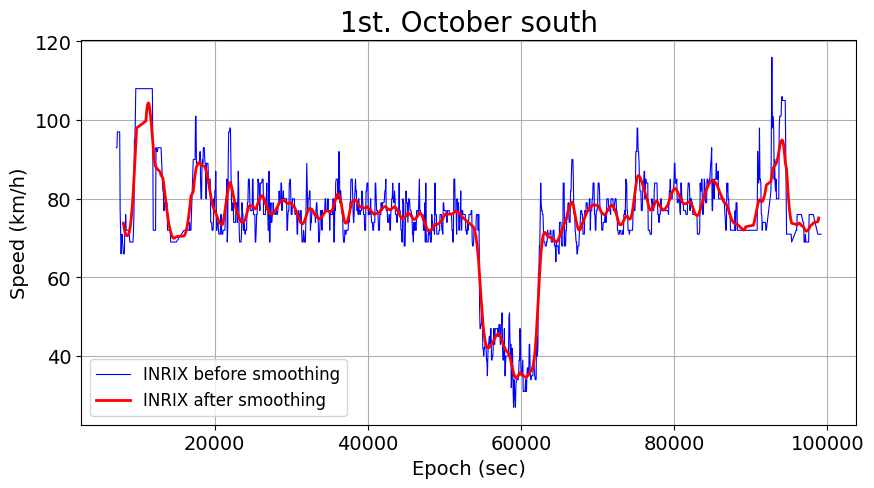
\includegraphics[width=\textwidth]{smoothing_inrix_speed.png}
        \caption{INRIX speed versus time (epoch) before and after smoothing.}
    \end{subfigure}
    \hfill
    \begin{subfigure}{0.7\textwidth}
        \centering
        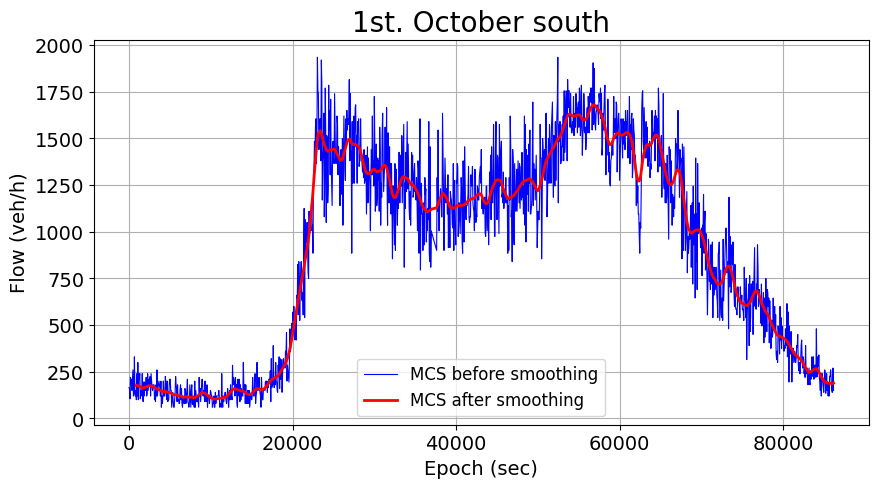
\includegraphics[width=\textwidth]{smoothing_mcs_flow.png}
        \caption{MCS flow versus time (epoch) before and after smoothing.}
    \end{subfigure}
    \caption{Time-series INRIX speed and MCS flow before and after smoothing on 1\textsuperscript{st} October.}
    \label{fig:smoothing}
\end{figure}

Figure~\ref{subfig:before_shifting} presents the INRIX speed and MCS speed versus epoch, i.e., cumulative time, based on their original timestamps. We can observe an approximate 6-minute latency of INRIX speed compared with the MCS speed from the figure, which is a common phenomenon reported by various studies related to the INRIX data [opportunity][KIM]. Since we aim to develop the relationship models that mapping the INRIX variables to the MCS flow and then use the models to estimate the traffic flow, we do not want any time difference between INRIX and MCS's observations. Therefore we shift the INRIX timestamps by 360 s to remove the time-lag between two measurements. Figure~\ref{subfig:after_shifting} presents the time-series INRIX and MCS speed after the timestamp shifting. We can see that the time-lag is disappeared, and the two curves overlap better after the shifting. By removing the latency, we ensure that both sensor platforms' measurements with the same timestamp reflect the same traffic condition at that moment.

\begin{figure}[!ht]
    \centering
    \begin{subfigure}{0.7\textwidth}
        \centering
        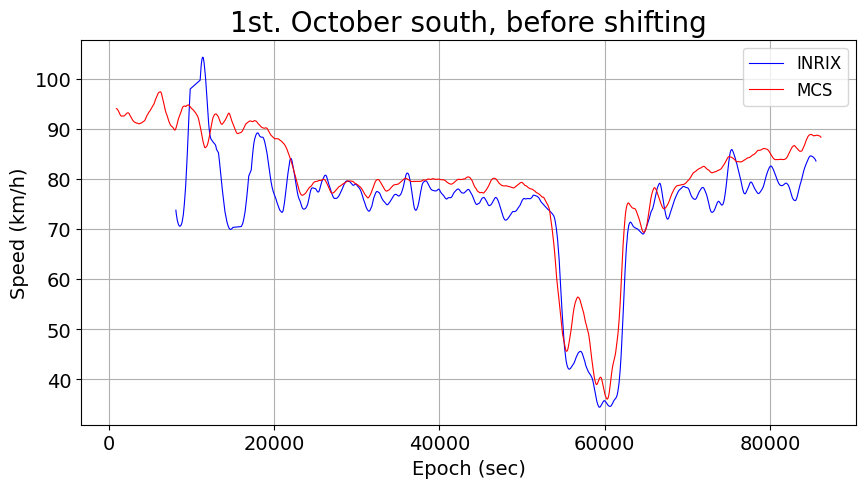
\includegraphics[width=\textwidth]{before_shifting.png}
        \caption{INRIX and MCS speed versus time based on original timestamps.}
        \label{subfig:before_shifting}
    \end{subfigure}
    \hfill
    \begin{subfigure}{0.7\textwidth}
        \centering
        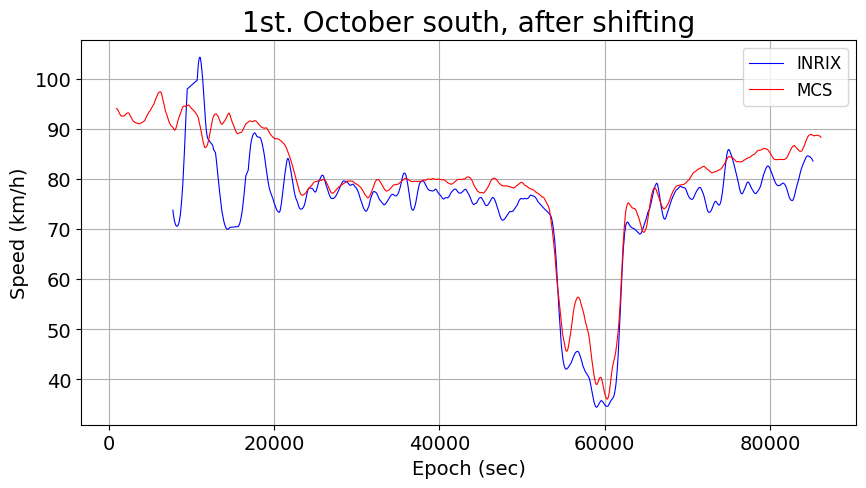
\includegraphics[width=\textwidth]{after_shifting.png}
        \caption{INRIX and MCS speed versus time after shifting INRIX timestamps with 360 s to remove the time-lag.}
        \label{subfig:after_shifting}
    \end{subfigure}
    \caption{INRIX and MCS speed versus time (epoch) before and after shifting INRIX timestamps on 1\textsuperscript{st} October.}
    \label{fig:shifting}
\end{figure}

Figure~\ref{fig:standardization_boxplots} presents box-plots showing the distributions of speed in the training and test datasets collected on both road segments before and after feature scaling, i.e., standardization. From figure~\ref{fig:standardization_boxplots}, we can see that the north segment's median speeds before the standardization are approximately 3 km slower than median speeds on the south segment, whether in the training sets or test sets. One reason for the lower median speed on the north road segment is that the north segment, compared with the south segment, is closer to Stockholm's city center, which generally has lower speed limits and more traffic than the city's outer parts. The interquartile ranges of the speed values are similar on both road segments. Figure ~\ref{fig:standardization_boxplots} also shows the distributions of standardized speeds in each dataset. We can see that the median values and the interquartile ranges on both road segments are similar. As standardization subtracts the historical mean speed value from the original speed value, the standardized speeds have a mean value close to zero. Thus the difference of median speed between the north and south segments is reduced. 

On the other hand, the distribution of speed in the test set is similar to the distribution in training set on the same segment, which means that the speed behavior did not change much in the short term future of one week.

\begin{figure}[!ht]
    \centering
    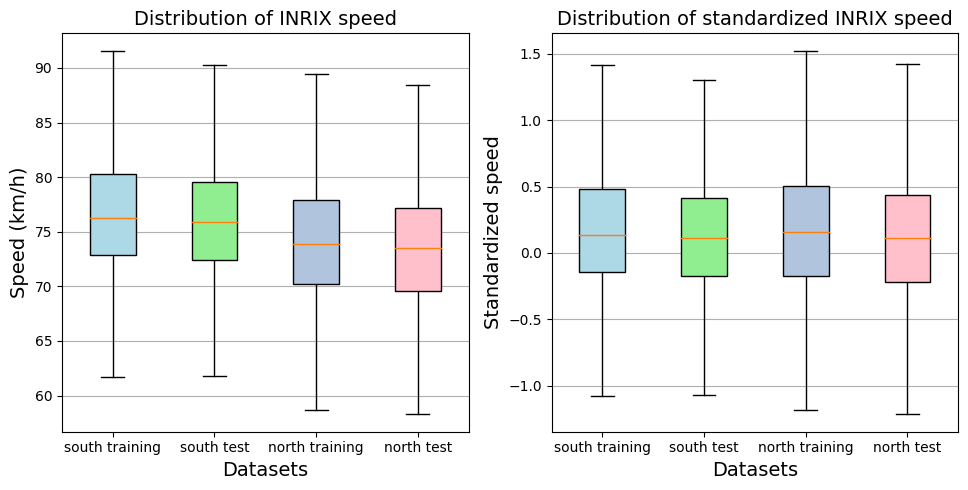
\includegraphics[width=\textwidth]{standardization_boxplots.png}
    \caption{Distributions of INRIX speed in training and test datasets before and after the standardization.}
    \label{fig:standardization_boxplots}
\end{figure}

\section{Model Training Results}
\label{sec:modelTrainingResults}

% baseline vs ANN flow-speed relationship

Figure~\ref{fig:base_ann_training} shows the baseline and the ANN flow-speed relationship trained on the samples from the south segment's training set. The samples used for training are also presented in the figure for comparison with the relationships.  To be noticed that the threshold speed separating the free-flow from the saturated regime for the baseline relationship in figure~\ref{fig:base_ann_training} is 70 km/h. The threshold speed was determined from the flow-density diagram using a regime identification method from \cite{nielsen_flow-speed_relations}. The density values were inferred from the flow and speed values using the equation~\ref{eq:basic_traffic_variable_relation}. Training errors for both models are shown in the table~\ref{tab:training_errors}.

\begin{figure}[!ht]
    \centering
    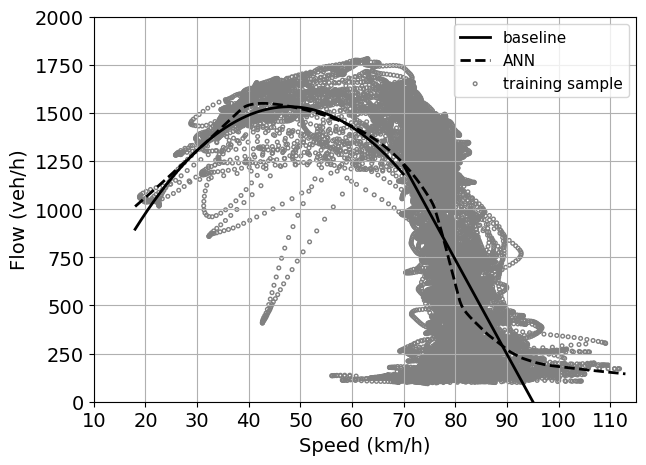
\includegraphics[width=0.8\textwidth]{baseline_ann_training.png}
    \caption{Baseline versus univariate ANN flow-speed relationship.}
    \label{fig:base_ann_training}
\end{figure}

\begin{table}[!ht]
\centering
\begin{tabular}{@{}lll@{}}
\toprule
\textbf{Training Error} & \textbf{Baseline Model} & \textbf{ANN Model} \\
\midrule
MAPE          & 96.49\% & 87.61\%    \\
RMSE          & 385.23  & 372.61     \\ 
\bottomrule
\end{tabular}
\caption{Training errors for baseline and univariate ANN flow-speed relationship model.}
\label{tab:training_errors}
\end{table}

Generally speaking, the ANN flow-speed relationship fits the training samples better than the baseline model, especially in the free-flow regime. From figure~\ref{fig:base_ann_training}, we can see that the baseline model uses linear regression to fit the samples in the free-flow regime, which is a common method for fitting the flow-speed relationship in free-flow regime \cite{blandin_individual_speed, nielsen_flow-speed_relations}. However, the flow-speed relationship in the free-flow regime is more S-shaped than linear in our dataset. ANN as a non-parametric model without fixed functional forms can adapt itself to the data and better fit the S-shaped flow-speed relationship in the free-flow regime. The ANN also has an advantage in the high-speed region, i.e., speed is larger than 90 km/h, where the traffic flow is low and barely changes with the speed.

% training results and temporal features for temporal ANN

Although the ANN can model the flow-speed relationship better than the baseline model, it does not mean that there is no space to improve our estimation model. In figure~\ref{fig:base_ann_training}, we can see that relationship between flow and speed is not deterministic; each speed value usually corresponds to a wide range of flow values in the samples. For example, when the speed is 80 km/h in the free-flow regime, the flow ranges from about 100 veh/h to 1500 veh/h, near eighty percent of the entire flow range! As we mentioned in the previous section, the flow-speed relationship varies over time rather than stationary. Thus, a deterministic curve could not capture the traffic flow variation given the same speed under different traffic conditions over time. One way to tackle this problem is to model the dynamic relationship using stochastic statistical models, e.g., Bayesian networks, which consider the transition between traffic conditions over time  \cite{neumann_bayesian}.

Another method to capture the dynamic flow-speed relationship on a road segment is to represent the flow-speed relationship as a time-varying function that considers temporal factors, e.g., time of a day, as features that affect the relationship curves. Figure~\ref{fig:temporalFactors} shows flow-speed behaviors of training samples in different time segments. In figure~\ref{fig:temporalFactor_a}, samples' distributions are different during different time segments of a day. For example, the traffic flow drops after 18:00 as compared with the earlier traffic states during the rush hours given the same speed. Weekdays and weekends also exhibit different behavior of flow-speed relationship. Figure~\ref{fig:temporalFactor_b} shows the training samples collected on Sunday (7\textsuperscript{th}) and Tuesday (9\textsuperscript{th}) on the same road segment. In figure~\ref{fig:temporalFactor_b}, we can see that the shape of relationship curves is different on the weekend from a weekday. The traffic flow on weekdays and weekends could significantly differ given the same speed in some time segments, e.g., morning.

\begin{figure}[!ht]
    \centering
    \begin{subfigure}{0.49\textwidth}
        \centering
        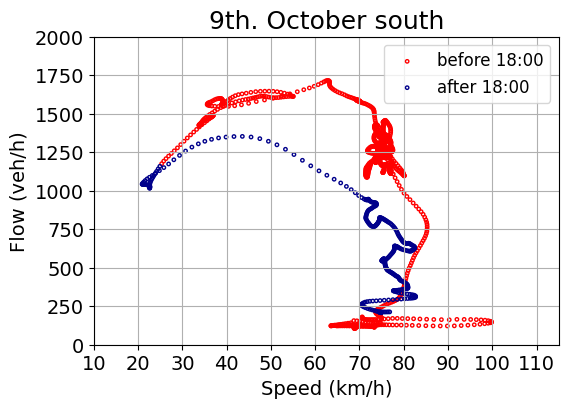
\includegraphics[width=\textwidth]{temporal_factors_a.png}
        \caption{Samples at different times of the day}
        \label{fig:temporalFactor_a}
    \end{subfigure}
    \hfill
    \begin{subfigure}{0.49\textwidth}
        \centering
        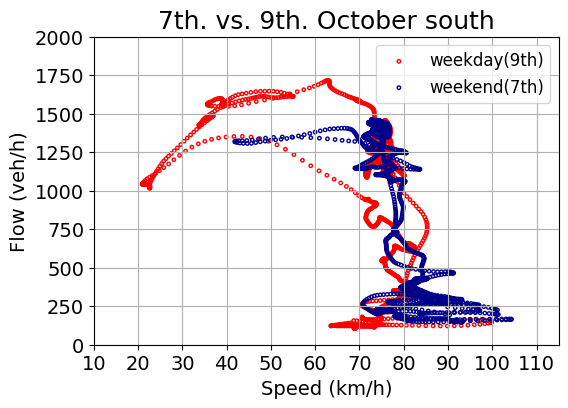
\includegraphics[width=\textwidth]{temporal_factors_b.png}
        \caption{Samples on the weekday and weekend.}
        \label{fig:temporalFactor_b}
    \end{subfigure}
    \caption{Training samples' different flow-speed behaviors in different time segments.}
    \label{fig:temporalFactors}
\end{figure}

By incorporating temporal factors as input features, we could train our ANN model to learn the dynamic flow-speed relationship over time. Figure~\ref{fig:temporal_ann_training} presents the trained ANN model considering temporal dependency, whose input features include speed and two time-related features, i.e., a 24-bit hour feature and a 2-bit day feature, as shown in equation~\ref{eq:temporal_ann_spd}. Instead of learning one static flow-speed relationship for the entire time, the temporal ANN learns many micro-relationships during training; each corresponds to a different time segment, i.e., a different hour of a day and a different day of a week. By incorporating additional time-related features, our ANN estimation model can capture traffic flow variation given the same speed to a certain degree. For example, the model will not provide only one estimated flow value when the speeds equal 80 km/h, but estimate the traffic flows according to which hour of a day and which day of a week sample's speeds are measured. Temporal ANN fits the training samples much better than the baseline and univariate ANN models, which are static flow-speed relationships. The temporal ANN's training MAPE is 11.54\%, and RMSE is 92.41. Most importantly, ANN learns and captures all micro-relationships for different time-segments automatically and efficiently without the need for human intervention or tedious codes for automation.

\begin{figure}[!ht]
    \centering
    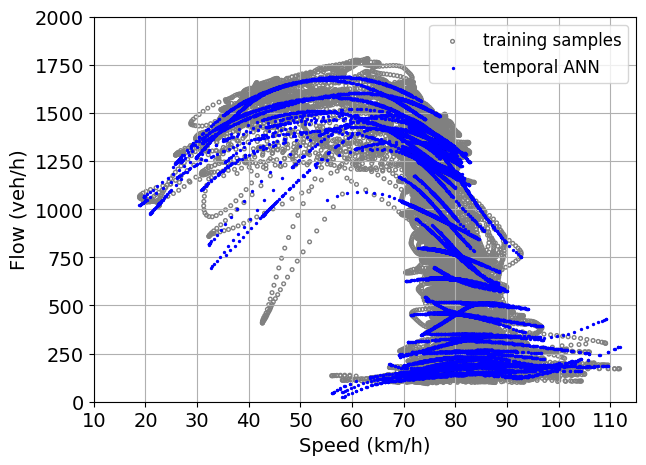
\includegraphics[width=0.8\textwidth]{temporal_ann_training.png}    \caption{Temporal ANN model considering flow-speed relationship's dependencies to the hour of a day and the day of a week.}
    \label{fig:temporal_ann_training}
\end{figure}

As mentioned in the previous section, the traffic condition depends on many factors, e.g., weather and lighting conditions, vehicle composition, road surface, and driver characteristics \cite{seo_tse, wang_tse_online_calibration}, all of which may affect the flow-speed relationship. Using temporal segmentation could not accurately capture the dynamic transitions between traffic conditions because they do not always occur during the changing of hours. Representing the traffic relationship as a time-varying function can also not reflect some causes leading to the changes of traffic conditions over time, e.g., percentage of the trucks. However, Incorporating the temporal dependency into the estimation model is a practical method to capture the dynamics of flow-speed relationships because it is difficult to explicitly monitor every factor on the road that affects the traffic conditions. We can see that this method effectively improves the model's training accuracy to a satisfactory level on a road segment whose traffic conditions are relatively ordinary and recurrent. In addition to the above models, we trained the other three ANN models mentioned in the section models using the training datasets. Each of the models incorporates additional features, i.e., travel time and location, for modeling the time-space-varying relationships between traffic state variables. In the next section, all estimation models are applied for estimating the traffic flows in unobserved time-space regions using the test datasets. Then we examine the overall performance obtained for each model.

\section{Traffic Flow Estimations}
\label{sec:trafficFlowEstimations}

Figure~\ref{fig:mape_histogram} represents the overview of the estimation performance in MAPE for all models when validated on the south and north test datasets collected in a week, i.e., 22\textsuperscript{nd} to 29\textsuperscript{th}, following the training dataset, i.e., 1\textsuperscript{st} to 21\textsuperscript{st}. However, before we start digging into each model's performance and comparing it with the baseline model, we observe a common phenomenon in the overall performance. 

\begin{figure}[!ht]
    \centering
    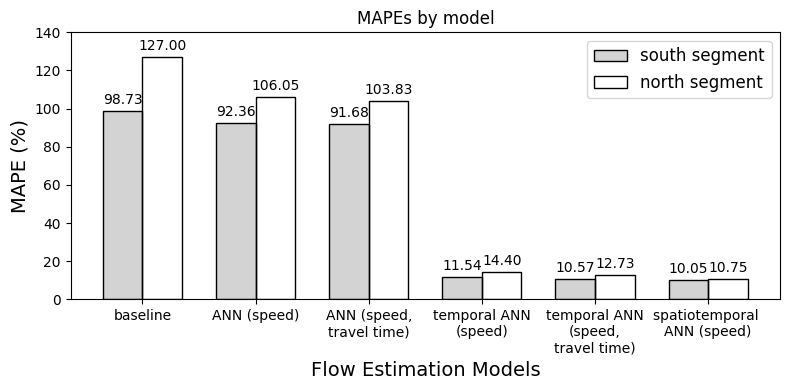
\includegraphics[width=\textwidth]{mape_histogram.png}
    \caption{Overview of the flow estimation performance on the two consecutive road segments.}
    \label{fig:mape_histogram}
\end{figure}

Models generally perform better on the south segment, where the models were trained, than on its consecutive adjacent segment, i.e., the north segment, except the spatiotemporal ANN model on the rightmost. For example, the baseline model has a smaller MAPE of 98.73\% on the south segment than the MAPE of 127.00\% on the north segment. The reason for the phenomenon is quite straightforward. As traffic conditions depend on many space-related factors \cite{seo_tse, wang_tse_online_calibration}, the traffic flow relationship on one segment may be slightly different from adjacent segments. Estimation models could perform well on the segment where they were trained as long as the traffic condition does not change much in the short-term future, e.g., one week in our case. However, they may not perform well on the adjacent segments because the adjacent segments' traffic flow relationships could be slightly different from those learned by the models. Therefore, the models produce more accurate estimations on the south segment than on the north segment. However, as shown in figure~\ref{fig:mape_histogram}, the degradation of estimation performance on the north segment could be mitigated using ANN as the estimation model, which will be discussed in detail later. On the other hand, the spatiotemporal ANN has similar MAPEs on both road segments because the model was trained on the samples from the both segments, which enable it to learn the unique traffic flow relationship for each segment.

The models in the figure~\ref{fig:mape_histogram} are presented from left to right with increasing complexity. The baseline model on the left is the simplest model with only one input feature, speed, and the spatiotemporal ANN on the rightmost is the most complex, having the most input features and model parameters. As shown in the figure, incorporating additional features and increasing the model complexity generally can improve the estimation performance on both segments. However, this trend is not always valid when evaluating the performance using RMSE, which we will see soon.

\begin{sidewaystable}
\centering
\begin{tabular}{@{}llllllllllll@{}}
\toprule
& Baseline & \multicolumn{4}{l}{ANN} & \multicolumn{4}{l}{Temporal ANN} & \multicolumn{2}{l}{Spatiotemporal ANN} \\
\cmidrule(lr){3-6} \cmidrule(lr){7-10} \cmidrule(lr){11-12}
& speed & \multicolumn{2}{l}{speed} & \multicolumn{2}{l}{speed, travel time} & \multicolumn{2}{l}{speed} & \multicolumn{2}{l}{speed, travel time} & \multicolumn{2}{l}{speed} \\
\cmidrule(lr){3-4} \cmidrule(lr){5-6} \cmidrule(lr){7-8} \cmidrule(lr){9-10} \cmidrule(lr){11-12}
& MAPE(\%) & MAPE & improv & MAPE & improv & MAPE & improv & MAPE & improv & MAPE & improv \\
\midrule
South & 98.73 & 92.36  & \textbf{6.4\%} & 91.68 & \textbf{7.1\%} & 11.54 & \textbf{88.3\%} & 10.57 & \textbf{89.3\%} & 10.05 & \textbf{89.8\%} \\
North & 127.00 & 106.05 & \textbf{16.5\%} & 103.83 & \textbf{18.2\%} & 14.40 & \textbf{88.7\%} & 12.73 & \textbf{90.0\%} & 10.75 & \textbf{91.5\%} \\
\bottomrule
\end{tabular}
\caption{Improvements of flow estimation performance (MAPE) achieved by ANN models over the baseline model.}
\label{tab:mape_imrpov}

\bigskip
\bigskip

\begin{tabular}{@{}llllllllllll@{}}
\toprule
& Baseline & \multicolumn{4}{l}{ANN} & \multicolumn{4}{l}{Temporal ANN} & \multicolumn{2}{l}{Spatiotemporal ANN} \\
\cmidrule(lr){3-6} \cmidrule(lr){7-10} \cmidrule(lr){11-12}
& speed & \multicolumn{2}{l}{speed} & \multicolumn{2}{l}{speed, travel time} & \multicolumn{2}{l}{speed} & \multicolumn{2}{l}{speed, travel time} & \multicolumn{2}{l}{speed} \\
\cmidrule(lr){3-4} \cmidrule(lr){5-6} \cmidrule(lr){7-8} \cmidrule(lr){9-10} \cmidrule(lr){11-12}
& RMSE(veh/h) & RMSE & improv & RMSE & improv & RMSE & improv & RMSE & improv & RMSE & improv \\
\midrule
South & 380.98 & 373.56  & \textbf{1.9\%} & 372.83 & \textbf{2.1\%} & 96.81 & \textbf{74.6\%} & 94.90 & \textbf{75.1\%} & 88.33 & \textbf{76.8\%} \\
North & 423.15 & 391.53 & \textbf{7.5\%} & 397.97 & \textbf{6.0\%} & 120.02 & \textbf{71.6\%} & 104.36 & \textbf{75.3\%} & 87.71 & \textbf{79.3\%} \\
\bottomrule
\end{tabular}
\caption{Improvements of flow estimation performance (RMSE) achieved by ANN models over the baseline model.}
\label{tab:rmse_imrpov}
\end{sidewaystable}

Tables \ref{tab:mape_imrpov} shows the improvements of ANN models as compared with the baseline model. We use the baseline model's MAPEs, i.e., 98.73\% on the south and 127.00\% on the north, as the reference performance to compare with the remaining ANN models. The ANN models can be categorized into three groups: The first group of ANNs considers only traffic variables, i.e., speed and travel time, as the independent variables without considering temporal or spatial dependency. The second group of ANNs considers temporal dependency in addition to the traffic variables, while the third group considers both the spatial and temporal dependency. The ANN using only speed as its independent variable has an improvement of 6.4\% on the south segment and 16.5\% on the north over the baseline model (south MAPE = 92.36\%, north MAPE = 106.05\%). Notice that ANN improves 10\% more on the north segment over the baseline case than on the south segment, which means ANN can mitigate the notable performance difference between adjacent segments when using the baseline model for estimation. The reason for ANN's better generality on the adjacent road segments will be discussed in the following section.The ANN incorporates the travel time as an additional independent variable reaches an improvement of 7.1\% on the south segment and 18.2\% on the north, which slightly improves the previous univariate ANN on both road segments. We will also discuss travel time as an additional input feature for flow estimation in the following section.

Incorporating temporal factors into flow estimation improves the performance considerably. As shown in the table~\ref{tab:mape_imrpov}, the temporal ANN, which uses speed and time-related features, i.e., hour and day, as its independent variables, dramatically improves 88.3\% on the south segment and 88.7\% on the north segment over the baseline's performance. The temporal ANN's errors are nearly one-tenth of that in the baseline model for both segments (south MAPE = 11.54\%, north MAPE = 14.40\%). The result validates our hypothesis that incorporating temporal dependency into flow estimation provides more information to the ANN and better captures the dynamic flow-speed relationship that changes over time. The temporal ANN with travel time as its additional information source also shows a slight improvement over the temporal ANN without using the travel time, which is similar to the static ANN models. Notice that the performance differences between two adjacent road segments still exist when using temporal ANNs for estimation, but they are much smaller than those in the static ANN models.

Finally, the spatiotemporal ANN, which incorporates time-related features, a space-related feature, and speed into flow estimation, achieves the best performance among all ANN models: a MAPE of 10.05\% on the south and a MAPE of 10.75\% on the north segment. It improves 89.8\% over the baseline model on the south and 91.5\% on the north. Spatiotemporal ANN not only has a negligible performance gap between the two road segments as we expected, but it also achieves a noticeable improvement on the south segment compared with the prior model scheme, i.e., temporal ANN (speed). Notice that the spatiotemporal ANN is the only model trained on the data from both road segments. We will discuss the spatial dependency and the benefits of using a spatiotemporal ANN in detail later.

Table~\ref{tab:rmse_imrpov} represents the overall estimation performance evaluated in RMSE for all models and the improvements achieved by ANN models compared with the baseline model. Although the values of improvements are different from the ones in MAPE, the overall trends of performance changes in RMSE are generally the same as the trends in MAPE regarding the changes made to the estimation model. However, one thing worth notice is that adding an additional source of traffic information, i.e., the travel time, into ANN models does not constantly improve the ANN's estimation performance in RMSE on the north segment. It could slightly degrade the ANN's performance on the north segment compared with the ANN without using the travel time. For example, in table \ref{tab:rmse_imrpov}, the ANN using both speed and travel time as independent variables only achieves 6.0\% improvement of RMSE on the north segment, which exhibits a decrement of 1.5\% compared with the ANN using speed as its sole information source.

Generally speaking, using the new ML technique, i.e., ANN, and incorporating additional dependencies or information sources, i.e., temporal dependency, spatial dependency, and travel time, into flow estimation improves the performance compared with the classic flow-speed relationship model. As we exhibited that improvements in MAPE can be as significant as 89.8\% on the south segment and 91.5\% on the north. The best performer, i.e., spatiotemporal ANN, improves 293 veh/h in RMSE (76.8\%) when used for traffic flow estimation on the south segment and 335 veh/h (79.3\%) on the north segment over the baseline model. ANN models generally achieve more improvements on the north segment than on the south segment. However, notice that travel time as an additional information source contributes only tiny improvements and could cause slight performance degradation on the north segment when evaluated using RMSE, which should be utilized with extra care.

\section{Discussion}
\label{sec:discussion}
This section analyzes and discusses some phenomena we observed in the results from the previous section. First of all, we will discuss why the ANN produces a better estimation performance on the adjacent road segment than the classic flow-speed relationship. Then we will discuss the role the travel time plays as an additional information source for flow estimation, e.g., why its benefit to the performance improvement is weak? Finally, we will shortly discuss what might happen when we incorporate spatial dependency into our ANN model and use data from multiple road segments for training. We also discuss what benefits it could bring us if we train a central estimation model that learns spatial dependency for the entire road network with many road segments.

\subsection{Generality}
\label{subsec:generality}

In the flow estimation results, the ANN using speed as the independent variable improves more performance, i.e., larger than 10\%, on the north segment than on the south segment. The result implies that the ANN model's performance degradation on the adjacent road segment is less severe than the baseline model's degradation. If a model can perform well on the road segments from which it has never seen data during the model training, we say it has good generality. Good generality of an estimation model is preferable because one of our goals is to use the model to estimate unobserved traffic flow on the road segments near the one where the model was trained. 

\begin{figure}[!ht]
    \centering
    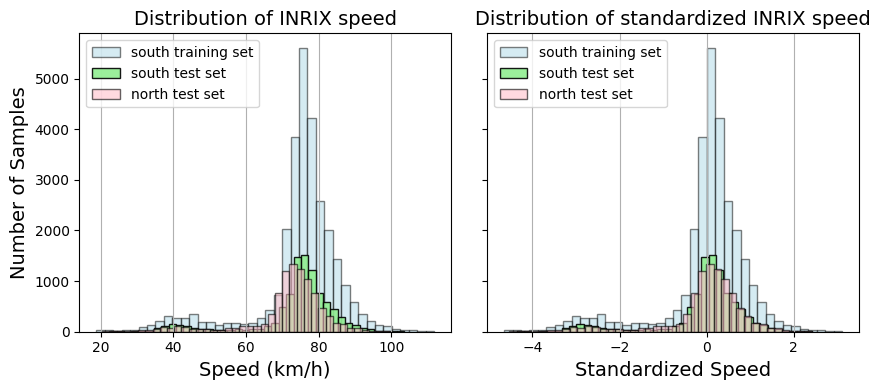
\includegraphics[width=1.0\textwidth]{speed_distribution_histogram.png}
    \caption{Distributions of input speed in the training and test datasets before and after the standardization for the ANN (speed) model.}
    \label{fig:distribution_histogram}
\end{figure}

However, why ANN model can perform more consistently on both road segments than the baseline model? We believe it is because ANN was trained on the scaled traffic variables rather than on traffic variables' original values. Remember the results of data preparation from the figure \ref{fig:standardization_boxplots}, the median speeds on the north segment are slower than the south segment. Figure \ref{fig:distribution_histogram} shows the speed distributions before and after the standardization in the training and test datasets for the baseline and ANN (speed) model. We can see in the figure that the distribution of speed on the north segment slightly shifts from the south segment's speed distribution to the left under the free-flow regime. The difference in free-flow speed between different road segments could be caused by many reasons, e.g., varying speed limits on different links \cite{neumann_bayesian}.


One reason for the baseline model's more severe performance degradation on the north segment is that we directly feed the north segment's speed into the flow-speed relationship as the evidence speed during the flow estimation. Notice that the flow-speed relationship in the baseline model was calibrated based on the south segment's speeds. The difference in speed distribution between two road segments could lead to the mismatch between the baseline flow-speed relationship and the flow-speed relationship lying in the samples observed on the north segment.

\begin{figure}[!ht]
    \centering
    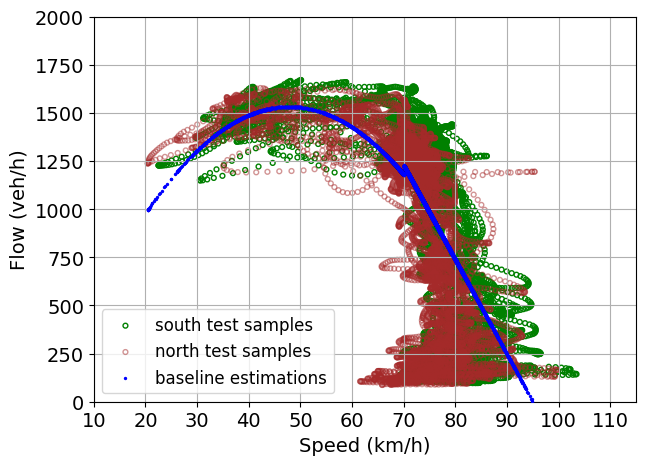
\includegraphics[width=0.8\textwidth]{relation_shift_baseline.png}
    \caption{Test samples from both road segments and corresponding flow estimations given by the baseline model.}
    \label{fig:relation_shift_baseline}
\end{figure}

Figure \ref{fig:relation_shift_baseline} shows the test data from both segments and the flow estimations produced by the baseline model based on the corresponding speeds. As shown in the figure, the baseline model uses the same flow-speed relationship, which was calibrated using the training speed from the south, to estimate the flow on both segments. However, since the flow-speed relationship lying in the north segment's test samples, which are brown circles, shifts to the left compared with the south segment's flow-speed relationship, the baseline relationship does not suit the actual relationship on the north segment as on the south segment. The baseline, therefore, suffers from a more noticeable performance degradation on the north segment.

On the other hand, the ANN model was trained on the south road segment's standardized speed. As mentioned before, we standardized the test datasets' speeds by subtracting the historical mean value, which was obtained from the training dataset on the same road segment, from the original speed values, then dividing the values by the historical standard deviation. As shown in the figure \ref{fig:distribution_histogram}, the distribution of standardized speeds on the north segment becomes similar to the south segment's speed distributions. The difference in speed between two segments under the free-flow regime is disappeared. Figure \ref{subfig:relation_shift_ann_standardized} shows the test samples from both segments and the corresponding flow estimations produced by the ANN model, all based on the standardized speeds. We can see that the relationships between flow and standardized speed on the neighboring road segments are similar. The ANN relationship trained on the south segment's standardized speed could also fit the relationship between flow and standardized speed on its adjacent road segments.  

\begin{figure}[!ht]
    \centering
    \begin{subfigure}{0.7\textwidth}
        \centering
        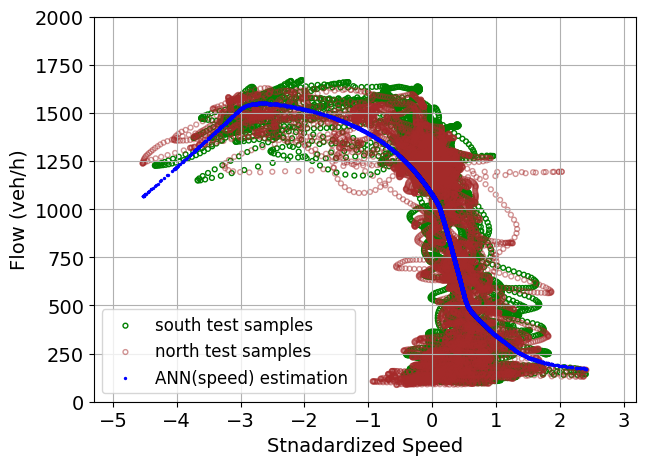
\includegraphics[width=\textwidth]{relation_shift_ann_a.png}
        \caption{Flow-speed diagram based on the standardized speed.}
        \label{subfig:relation_shift_ann_standardized}
    \end{subfigure}
    \hfill
    \begin{subfigure}{0.7\textwidth}
        \centering
        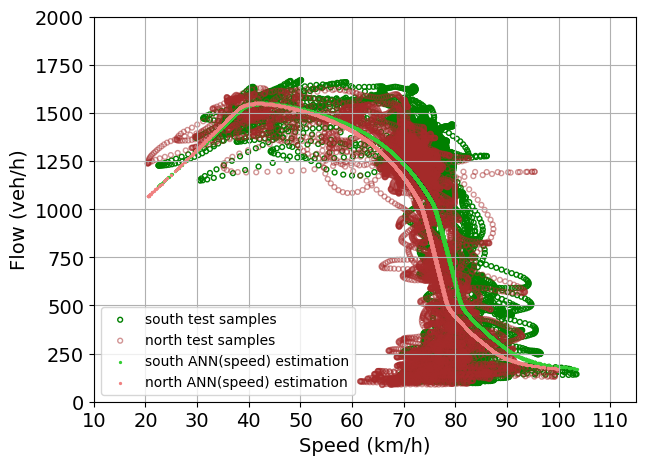
\includegraphics[width=\textwidth]{relation_shift_ann_b.png}
        \caption{Flow-speed diagram based on the original speed.}
        \label{subfig:relation_shift_ann_raw}
    \end{subfigure}
    \caption{Test samples from both road segments and the corresponding flow estimations given by the ANN (speed) model.}
    \label{fig:relation_shift_ann}
\end{figure}

Figure \ref{subfig:relation_shift_ann_raw} shows the test samples on the two road segments and corresponding ANN model's estimations based on the actual speeds. The ANN model seems to adapt to the speed change under the free-flow regime and split into two flow-speed relationships to fit each segment's samples. In conclusion, standardization of features gives ANNs better resistance to speed differences between adjacent road segments. Although the ANN model is still far from a fully general model, it has better generality on neighboring road segments than the traditional flow-speed relationship.

\subsection{Travel Time}
\label{subsec:discussionTravelTime}

As mentioned before, INRIX data, which is a kind of mobile data collected from probe vehicles, calculate the speed as the average speed of vehicles over a length of the road, which is called space mean speed \cite{sharma_inrix_data_opportunity, Ahsani_inrix_data_quantity}. Space mean speed can be calculated as following equation \cite{elefteriadou_traffic_flow_theory}:

\begin{equation}
    v_{avg} = \frac{d}{\frac{1}{n}\sum_{1}^{n}t_{i}}
    \label{eq:sms}
\end{equation}
\begin{align*}
    & d = the \ distance \ over \ which \ travel \ times \ were \ measured\\ 
    & t_i = the \ travel \ time \ measured \ for \ the \ i^{th} \ vehicle
\end{align*}

The denominator in equation \ref{eq:sms} is the average travel time that vehicles take to travel across the road segment reported by the INRIX platform. Therefore, according to the equation, the INRIX speed and travel time are only two variables inversely proportional to each other. Figure \ref{fig:speed_vs_travel_time} shows the relationship between speed and travel time in the south segment's training dataset. Although there are some variations in the data, we can see that the relationship between speed and travel time is indeed an inverse proportion. Based on this fact, we did not expect that the travel time would provide additional helpful information than the speed in flow estimation.

\begin{figure}[!ht]
    \centering
    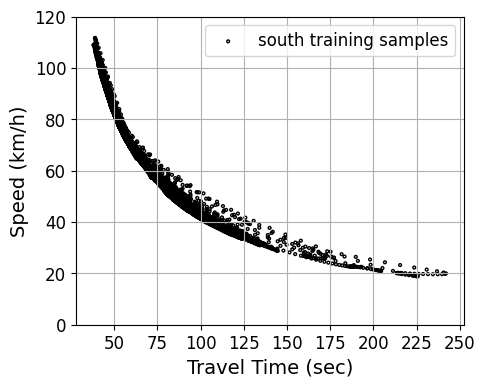
\includegraphics[width=0.6\textwidth]{speed_vs_travel_time.png}
    \caption{Relationship between speed and travel time in the training dataset from the south road segment.}
    \label{fig:speed_vs_travel_time}
\end{figure}

However, adding travel time still improves the estimation performance slightly, as we demonstrated in section \ref{sec:trafficFlowEstimations}. One possible reason is that travel time as an additional feature may complement speed when the speed value is small. As shown in figure \ref{fig:speed_vs_travel_time}, when the speed is small, e.g., below 40 km/h, the speed changes are also small. On the other hand, changes in travel times under this regime are more pronounced, providing additional information for the model to recognize different traffic states and flows. Nevertheless, the improvement that travel time could bring is slight compared to other techniques such as temporal dependency.

\begin{figure}[!ht]
    \centering
    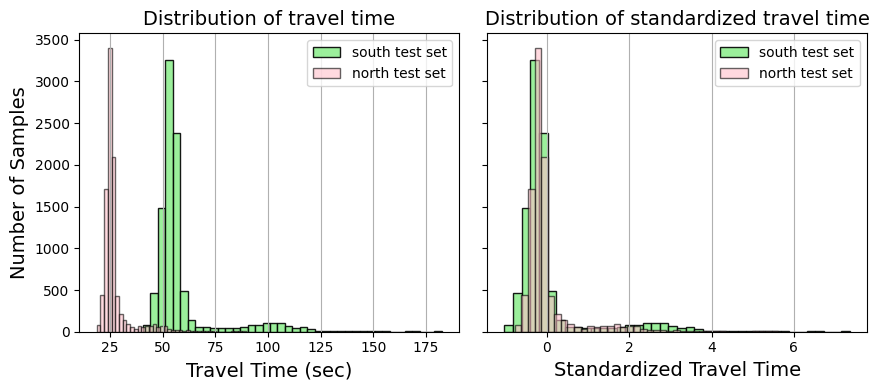
\includegraphics[width=1.0\textwidth]{ttime_distribution_histogram.png}
    \caption{Distributions of travel time in the test datasets before and after the standardization.}
    \label{fig:travel_time_distribution_histogram}
\end{figure}

As we demonstrated in the result of flow estimation, travel time could sometimes worsen the model's performance on the adjacent road segment instead of improving it. After examining the datasets on the north segment between 1\textsuperscript{st} and 21\textsuperscript{nd} October, we found some severe congestions occurred on the north segment but not south. The severe congestions resulted in some high travel times, which could be as large as ten times the median travel time. The high values affect travel time's distribution on the north segment, leading to the different distributions between two road segments after the standardization. Because our ANN (speed, travel time) model was trained based on the standardized travel times from the south segment without experiencing severe congestions, there will be a slight mismatch between the trained ANN relationship and the north's relationship. This mismatch causes the performance deterioration on the north segment, similar to the baseline model case.  The difference is that this time the standardization cannot eliminate the fundamental difference in travel time distribution between two road segments caused by the congestions. Figure \ref{fig:travel_time_distribution_histogram} shows the distributions of travel times in both segments' test datasets before and after the standardization. As shown in the figure, the difference in travel time distribution between two road segments, i.e., the different standard deviations, still exists after the standardization.

In contrast, speed as an information source for estimation is less affected by congestions. Theoretically, while the travel time could increase fast and unlimitedly as the congestion piles up, the speed changes relatively little and has a minimum value of 0 km/h. Therefore, the speed distribution is less affected by the congestions, and the standardized speeds are similar on the adjacent road segment, as shown in figure \ref{fig:distribution_histogram}. In conclusion, the speed is a better choice of information source for flow estimation than the travel time because the traffic flow relationship trained on the standardized speeds is less affected by the variations in traffic conditions, and it consistently fits the samples on different road segments.

\subsection{Spatial Dependency}
\label{subsec:discussionSpatialDependency}

As we demonstrated in the flow estimation results, when we incorporated the spatial dependency into flow estimation, the performance gaps observed in all other estimation models between the south and north segments disappear. Because we trained the spatiotemporal ANN using data from both road segments and adopted a location feature for identifying each segment, the model could learn the unique characteristics of the time-varying traffic flow relationship on the north segment, just like it did on the south. Thus the spatiotemporal ANN achieves a consistent performance on both segments. 

\begin{figure}[!ht]
    \centering
    \begin{subfigure}{0.49\textwidth}
        \centering
        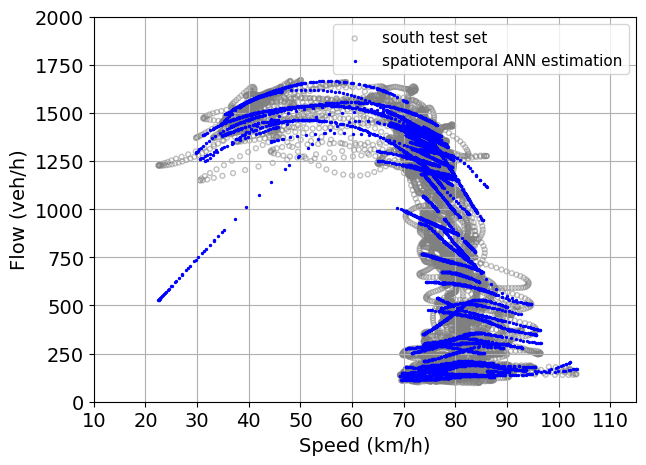
\includegraphics[width=\textwidth]{spatiotemporal_ann_south.png}
        \caption{Estimations and test samples on the south segment.}
        \label{subfig:spatiotemporal_ann_south}
    \end{subfigure}
    \hfill
    \begin{subfigure}{0.49\textwidth}
        \centering
        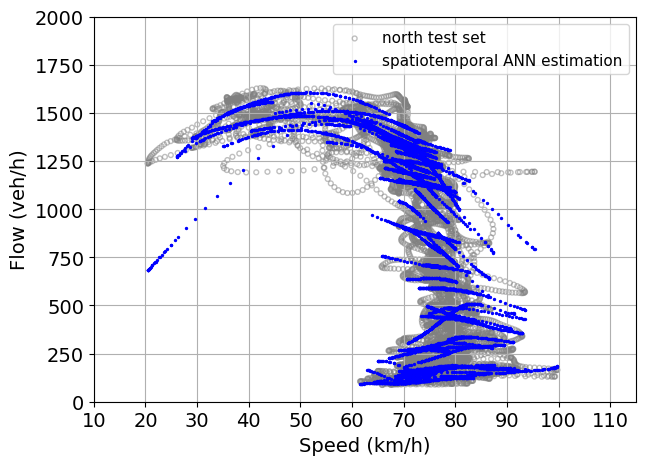
\includegraphics[width=\textwidth]{spatiotemporal_ann_north.png}
        \caption{Estimations and test samples on the north segment.}
        \label{subfig:spatiotemporal_ann_north}
    \end{subfigure}
    \caption{Spatiotemporal ANN's flow estimations on both road segments.}
    \label{fig:spatiotemporal_ann}
\end{figure}

However, to our surprise, considering the spatial dependency not only improves the performance on the adjacent road segment but also achieves a noticeable improvement on the south segment compared with the temporal ANN. For example, as shown in table MAPE and table RMSE, the spatiotemporal ANN achieves 1.6\% more improvement in MAPE and 2.2\% more improvements in RMSE on the south segment relative to the temporal ANN (speed), which does consider the spatial dependency. Our explanation for this improvement on the south segment is that the exploitation of data from multiple road segments may provide the ANN model with more traffic data patterns. That additional information helps the ANN learn a more comprehensive and universal flow-speed relationship and better estimate the traffic flows on the south segment than the model trained on data from only one segment. One indirect evidence for the explanation could be found in figure \ref{fig:spatiotemporal_ann}, which presents the spatiotemporal ANN's flow estimations and the test samples for both segments. Although there are deformation and position differences between the two estimations in the flow-speed diagrams, e.g., the relationship curve's height is smaller on the north segment than on the south. We can see that the time-varying flow-speed relationships given by the spatiotemporal ANN on both segments are very similar. Considering there are only 120 parameters corresponding to the model's location feature, the model cannot learn an entirely new time-varying relationship for each segment. Spatiotemporal ANN more likely learned a universal time-varying flow-speed relationship shared by both segments and captured each segment's relationship's unique characteristics according to their location feature, e.g., shorten the height of the relationship curve for the north segment. Thus more training data improves the universal relationship shared by both segments and further improves the model's performance on the south segment. Unfortunately, it is not easy to analyze how spatiotemporal ANN works internally and prove our explanation's correctness since the ANN is a black-box model.

We can, of course, build and train many small ANN models for estimating flows on road segments in a network instead of building an ANN considering spatial dependency. However, spatiotemporal ANN shows the possibility of a central estimation model that learns the spatiotemporal dependencies for the entire road network and might provide some benefits over single segment models. First, it could reduce the number of estimation models needed by ITS for estimating the traffic flow in a road network. A central estimation model will have fewer parameters than the combination of many small models, a more efficient way to model the traffic dynamics in a transportation system with many road segments. Second, as we discussed above, training a model using data from multiple road segments might improve the overall performance on every road segment covered by the model compared with using data from a single road segment for training. Because the central estimation model is more complex than the single segment model, it might also suffer from long training and computational time. However, we need to validate spatiotemporal ANN's performance and benefits when building a central estimation model on a road network with many road segments via network-wide sensor data.

\subsection{Usage of Estimation Model and Model Update}
\label{subsec:discussionModelUsage}

Finally, we shortly discuss the use of ANN models proposed in this work for flow estimation/imputation and the update of models over time. 

The situation is simple when we use the ANN models to impute the missing data due to fixed sensor malfunctions or communication failures on the road segments. We use the ANN model trained on the historical data, i.e., data in the training set, to impute the missing flow data on the same road segment where the model was trained. The case is similar to what we did when using the ANN models trained on  E4's south road segment to estimate the traffic flow on the same segment between 22\textsuperscript{nd} and 28\textsuperscript{th} October.

However, when we intend to use the models for estimating the traffic flow on the road segments and regions where there is no fixed sensor installed and the traffic flow is never observed, the situation is more complex than the imputation. We knew that the training of a model strongly depends on many factors, e.g., number of lanes, speed limit, road surface, road's geometric alignment, road type, and much more \cite{seo_tse, neumann_bayesian}, all of which may affect the traffic flow characteristics on a road, e.g., capacity and free-flow speed. Thus, a model trained on one road segment may not be suitable for another road segment with different traffic flow characteristics. Using an inappropriate model for estimation will lead to erroneous results.

When our goal is to estimate the traffic flow on the road segments between two adjacent fixed sensors, as shown in figure \ref{fig:tse}, the situation is relatively simple. We assume that a segment's traffic characteristics do not change much from the nearest sensor locations because the usual space between sensors is only several hundred meters to few kilometers. Based on the assumption, we have two alternative approaches to choose the model for estimating the flow on the road segment. The first approach is choosing the ANN model trained on the physically nearest road segment with the fixed sensor installed. For example, in this project, we estimated the flow on E4's north road segment using temporal ANN models trained on its nearest road segment with a fixed sensor, i.e., the south segment in the distance of 1 km. As we demonstrated, the models produced satisfied estimation results on the north segment, whose performance is only slightly worse than that on the south segment. Note that in the case of using spatiotemporal ANN, we assign the nearest fixed sensor's location feature to the evidence data samples on the target segment to select the traffic flow relationship to be used.

\begin{figure}[!ht]
    \centering
    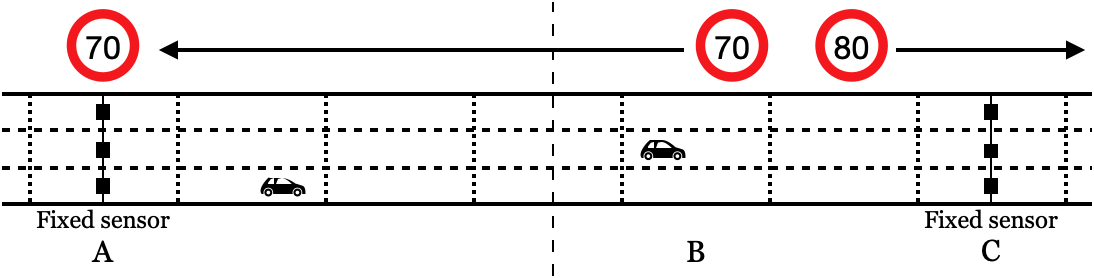
\includegraphics[width=1.0\textwidth]{speed_limit_transition.png}
    \caption{Conceptual representation for a road segment between two fixed sensors with a speed limit transition.}
    \label{fig:speed_limit_transition}
\end{figure}

However, the first approach could lead to a problem that the nearest segment might not have the most similar traffic flow characteristics as the target road segment. Figure estimation shows an example for this problem. In figure estimation, road segment B between fixed sensor segment A and C is the target segment for estimating the flow. Although B is closer to the C segment, B's speed limit is the same as A's speed limit. As we discussed in the previous sections, different speed limits and probably other factors might cause different speed distributions, resulting in different traffic flow characteristics on different road segments. Therefore, using the C segment estimation model, which has the nearest fixed sensor and a speed limit of 80 km/h, might not be a better choice than choosing the A segment's model in this case. To solve this problem, we propose a second approach is to choose the estimation model from the road segment that has a similar speed distribution, i.e., standard deviation and mean speed, as the target road segment out of the nearest two segments with fixed sensors.

On the other hand, if we want to use the trained models to estimate the flows for road segments on different roads in a road network or on the same roads but far from where the models were trained, the problem will be much more complicated. The traffic flow characteristics on those target road segments could be very different from the segments where the models trained. We could adopt an approach proposed by Neumann et al. \cite{neumann_bayesian} for this use case. According to Neumann, first, we need to identify a scheme of factors, e.g., number of lanes, speed limit, road type, that affect the traffic flow characteristics. Based on the scheme, we group all roads into several classes. The roads within a class have similar traffic characteristics. Finally, we train an estimation model on one road segment for each class and estimate the flow on the same class's road segments using this model. By adopting this approach, estimation models' usage will not be confined to the regions in proximity to fixed sensors anymore.
Moreover, we could use it in a geographically broader region in a road network. However, identifying the factors that affect traffic flow characteristics and developing a practical scheme for classifying homogenous road classes is difficult. It is hence out of this thesis's scope. Nevertheless, ANN's ability to learn complex relationships in the high dimensional dataset, as we have shown in this work, still makes it a competitive candidate when building a more general model that incorporates all influential factors into flow estimation in a road network.

Finally, we need to regularly update and retrain our estimation models using the new observed dataset once deployed in ITS. As a common phenomenon in machine learning, almost all the models degrade over time, so do our estimation models. For example, the ANN model trained before the lockdown will probably perform poorly once the government implements a lockdown due to the 2020 pandemic. The driver's behavior in rush hours will be very different when people start to work from home. Therefore, regularly monitor the model and retrain it with the newly updated datasets is very important to ensure that the model can learn the new traffic flow characteristics and its performance does not drop. Fortunately, automating the processes of building and training the machine learning models we proposed is very simple because our approach is highly automated. One only needs to regularly run the script we provided in the Github repository to build and train the estimation models, for example, every week using updated data via some common scheduling commands in Unix.


\cleardoublepagepage









































\chapter{What you did}\todo[inline]{Choose your own chapter title to describe this}
\todo[inline, backgroundcolor=aqua]{[Vad gjorde du? Hur gick det till? – Välj lämplig rubrik (“Genomförande”, “Konstruktion”, ”Utveckling”  eller annat]}
\label{ch:whatYouDid}

\todo[inline]{What have you done? How did you do it? What design decisions did you make? How did what you did help you to meet your goals?}
\begin{swedishnotes}
Vad du har gjort? Hur gjorde du det? Vad designen beslut gjorde du?
Hur kom det du hjälpte dig att uppnå dina mål?
\end{swedishnotes}

\section{Hardware/Software design …/Model/Simulation model \& parameters/…}
\todo[inline, backgroundcolor=aqua]{Hårdvara / Mjukvarudesign ... / modell / Simuleringsmodell och parametrar / …}

Figure~\ref{fig:homepageicon} shows a simple icon for a home page. The time
to access this page when served will be quantified in a series of
experiments. The configurations that have been tested in the test bed are
listed in Table~\ref{tab:configstested}.

\begin{swedishnotes}
Figur~\ref{fig:homepageicon}  visar en enkel ikon för en hemsida. Tiden för att få tillgång till den här sidan när serveras kommer att kvantifieras i en serie experiment. De konfigurationer som har testats i provbänk listas ini tabell~\ref{tab:configstested}.

Vad du har gjort? Hur gjorde du det? Vad designen beslut gjorde du?
\end{swedishnotes}
 
\begin{figure}[!h]
  \begin{center}
    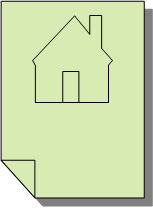
\includegraphics[width=0.25\textwidth]{Homepage-icon.png}
  \end{center}
  \caption{Homepage icon}
  \label{fig:homepageicon}
\end{figure}

\begin{table}[!ht]
  \begin{center}
    \caption{Configurations tested}
    \label{tab:configstested}
    \begin{tabular}{l|c} % <-- Alignments: 1st column left, 2nd middle and 3rd right, with vertical lines in between
      \textbf{Configuration} & \textbf{Description} \\
      \hline
      1 & Simple test with one server\\
      2 & Simple test with one server\\
    \end{tabular}
  \end{center}
\end{table}
\todo[inline, backgroundcolor=aqua]{Konfigurationer testade}

\section{Implementation …/Modeling/Simulation/…}
\todo[inline, backgroundcolor=aqua]{Implementering … / modellering / simulering / …}
\label{sec:implementationDetails}

\subsection{Some examples of coding}

Listing~\ref{lst:helloWorldInC} shows an example of a simple program written
in C code.

\begin{lstlisting}[language={C}, caption={Hello world in C code}, label=lst:helloWorldInC]
int main() {
printf("hello, world");
return 0;
}
\end{lstlisting}


In contrast, Listing~\ref{lst:programmes} is an example of code in Python to
get a list of all of the programs at KTH.

\lstset{extendedchars=true}
\begin{lstlisting}[language={Python}, caption={Using a python program to
    access the KTH API to get all of the programs at KTH}, label=lst:programmes]
KOPPSbaseUrl = 'https://www.kth.se'

def v1_get_programmes():
    global Verbose_Flag
    #
    # Use the KOPPS API to get the data
    # note that this returns XML
    url = "{0}/api/kopps/v1/programme".format(KOPPSbaseUrl)
    if Verbose_Flag:
        print("url: " + url)
    #
    r = requests.get(url)
    if Verbose_Flag:
        print("result of getting v1 programme: {}".format(r.text))
    #
    if r.status_code == requests.codes.ok:
        return r.text           # simply return the XML
    #
    return None
\end{lstlisting}


\cleardoublepage
\chapter{Results and Discussion}
\todo[inline, backgroundcolor=aqua]{svensk: Resultat och Analys}
\label{ch:resultsAndDiscussion}
\todo[inline]{
Sometimes this is split into two chapters.\\
  
Keep in mind: How you are going to evaluate what you have done? What are your metrics?\\
Analysis of your data and proposed solution\\
Does this meet the goals which you had when you started?
}

In this chapter, we present the results and discuss them.

\begin{swedishnotes}
I detta kapitel presenterar vi resultatet och diskutera dem.
\end{swedishnotes}
\todo[inline, backgroundcolor=aqua]{
Ibland delas detta upp i två kapitel.\\
Hur du ska utvärdera vad du har gjort? Vad är din statistik?\\
Analys av data och föreslagen lösning\\
Innebär detta att uppnå de mål som du hade när du började?
}

\section{Major results}
\todo[inline, backgroundcolor=aqua]{Huvudsakliga resultat}

Some statistics of the delay measurements are shown in Table~\ref{tab:delayMeasurements}.
The delay has been computed from the time the GET request is received until the response is sent.

\begin{swedishnotes}
Lite statistik av mätningarna fördröjnings visas i Tabell~\ref{tab:delayMeasurements}. Förseningen har beräknats från den tidpunkt då begäran GET tas emot fram till svaret skickas.
\end{swedishnotes}

\begin{table}[!ht]
  \begin{center}
    \caption{Delay measurement statistics}
    \label{tab:delayMeasurements}
    \begin{tabular}{l|S[table-format=4.2]|S[table-format=3.2]} % <-- Alignments: 1st column left, 2nd middle and 3rd right, with vertical lines in between
      \textbf{Configuration} & \textbf{Average delay (ns)} & \textbf{Median delay (ns)}\\
      \hline
      1 & 467.35 & 450.10\\
      2 & 1687.5 & 901.23\\
    \end{tabular}
  \end{center}
\end{table}
\todo[inline, backgroundcolor=aqua]{Fördröj mätstatistik}
\todo[inline, backgroundcolor=aqua]{Konfiguration | Genomsnittlig fördröjning (ns) | Median fördröjning (ns)}

Figure \ref{fig:processing_vs_payload_length} shows and example of the
performance as measured in the experiments.

\begin{figure}[!ht]
% GNUPLOT: LaTeX picture
\setlength{\unitlength}{0.240900pt}
\ifx\plotpoint\undefined\newsavebox{\plotpoint}\fi
\begin{picture}(1500,900)(0,0)
\sbox{\plotpoint}{\rule[-0.200pt]{0.400pt}{0.400pt}}%
\put(171.0,131.0){\rule[-0.200pt]{4.818pt}{0.400pt}}
\put(151,131){\makebox(0,0)[r]{ 1.5}}
\put(1419.0,131.0){\rule[-0.200pt]{4.818pt}{0.400pt}}
\put(171.0,212.0){\rule[-0.200pt]{4.818pt}{0.400pt}}
\put(151,212){\makebox(0,0)[r]{ 2}}
\put(1419.0,212.0){\rule[-0.200pt]{4.818pt}{0.400pt}}
\put(171.0,292.0){\rule[-0.200pt]{4.818pt}{0.400pt}}
\put(151,292){\makebox(0,0)[r]{ 2.5}}
\put(1419.0,292.0){\rule[-0.200pt]{4.818pt}{0.400pt}}
\put(171.0,373.0){\rule[-0.200pt]{4.818pt}{0.400pt}}
\put(151,373){\makebox(0,0)[r]{ 3}}
\put(1419.0,373.0){\rule[-0.200pt]{4.818pt}{0.400pt}}
\put(171.0,454.0){\rule[-0.200pt]{4.818pt}{0.400pt}}
\put(151,454){\makebox(0,0)[r]{ 3.5}}
\put(1419.0,454.0){\rule[-0.200pt]{4.818pt}{0.400pt}}
\put(171.0,534.0){\rule[-0.200pt]{4.818pt}{0.400pt}}
\put(151,534){\makebox(0,0)[r]{ 4}}
\put(1419.0,534.0){\rule[-0.200pt]{4.818pt}{0.400pt}}
\put(171.0,615.0){\rule[-0.200pt]{4.818pt}{0.400pt}}
\put(151,615){\makebox(0,0)[r]{ 4.5}}
\put(1419.0,615.0){\rule[-0.200pt]{4.818pt}{0.400pt}}
\put(171.0,695.0){\rule[-0.200pt]{4.818pt}{0.400pt}}
\put(151,695){\makebox(0,0)[r]{ 5}}
\put(1419.0,695.0){\rule[-0.200pt]{4.818pt}{0.400pt}}
\put(171.0,776.0){\rule[-0.200pt]{4.818pt}{0.400pt}}
\put(151,776){\makebox(0,0)[r]{ 5.5}}
\put(1419.0,776.0){\rule[-0.200pt]{4.818pt}{0.400pt}}
\put(171.0,131.0){\rule[-0.200pt]{0.400pt}{4.818pt}}
\put(171,90){\makebox(0,0){ 0}}
\put(171.0,756.0){\rule[-0.200pt]{0.400pt}{4.818pt}}
\put(298.0,131.0){\rule[-0.200pt]{0.400pt}{4.818pt}}
\put(298,90){\makebox(0,0){ 10}}
\put(298.0,756.0){\rule[-0.200pt]{0.400pt}{4.818pt}}
\put(425.0,131.0){\rule[-0.200pt]{0.400pt}{4.818pt}}
\put(425,90){\makebox(0,0){ 20}}
\put(425.0,756.0){\rule[-0.200pt]{0.400pt}{4.818pt}}
\put(551.0,131.0){\rule[-0.200pt]{0.400pt}{4.818pt}}
\put(551,90){\makebox(0,0){ 30}}
\put(551.0,756.0){\rule[-0.200pt]{0.400pt}{4.818pt}}
\put(678.0,131.0){\rule[-0.200pt]{0.400pt}{4.818pt}}
\put(678,90){\makebox(0,0){ 40}}
\put(678.0,756.0){\rule[-0.200pt]{0.400pt}{4.818pt}}
\put(805.0,131.0){\rule[-0.200pt]{0.400pt}{4.818pt}}
\put(805,90){\makebox(0,0){ 50}}
\put(805.0,756.0){\rule[-0.200pt]{0.400pt}{4.818pt}}
\put(932.0,131.0){\rule[-0.200pt]{0.400pt}{4.818pt}}
\put(932,90){\makebox(0,0){ 60}}
\put(932.0,756.0){\rule[-0.200pt]{0.400pt}{4.818pt}}
\put(1059.0,131.0){\rule[-0.200pt]{0.400pt}{4.818pt}}
\put(1059,90){\makebox(0,0){ 70}}
\put(1059.0,756.0){\rule[-0.200pt]{0.400pt}{4.818pt}}
\put(1185.0,131.0){\rule[-0.200pt]{0.400pt}{4.818pt}}
\put(1185,90){\makebox(0,0){ 80}}
\put(1185.0,756.0){\rule[-0.200pt]{0.400pt}{4.818pt}}
\put(1312.0,131.0){\rule[-0.200pt]{0.400pt}{4.818pt}}
\put(1312,90){\makebox(0,0){ 90}}
\put(1312.0,756.0){\rule[-0.200pt]{0.400pt}{4.818pt}}
\put(1439.0,131.0){\rule[-0.200pt]{0.400pt}{4.818pt}}
\put(1439,90){\makebox(0,0){ 100}}
\put(1439.0,756.0){\rule[-0.200pt]{0.400pt}{4.818pt}}
\put(171.0,131.0){\rule[-0.200pt]{0.400pt}{155.380pt}}
\put(171.0,131.0){\rule[-0.200pt]{305.461pt}{0.400pt}}
\put(1439.0,131.0){\rule[-0.200pt]{0.400pt}{155.380pt}}
\put(171.0,776.0){\rule[-0.200pt]{305.461pt}{0.400pt}}
\put(30,453){\rotatebox{-270}{\makebox(0,0){Processing time (ms)}}}
\put(805,29){\makebox(0,0){Payload size (bytes)}}
\put(868.0,131.0){\rule[-0.200pt]{0.400pt}{84.074pt}}
\put(995.0,131.0){\rule[-0.200pt]{0.400pt}{98.287pt}}
\put(1173.0,131.0){\rule[-0.200pt]{0.400pt}{118.041pt}}
\put(1325.0,131.0){\rule[-0.200pt]{0.400pt}{134.904pt}}
\put(1350.0,131.0){\rule[-0.200pt]{0.400pt}{137.795pt}}
\put(1439.0,131.0){\rule[-0.200pt]{0.400pt}{155.380pt}}
\end{picture}
\caption[A GNUplot figure]{Processing time vs. payload length}\vspace{0.5cm}
\label{fig:processing_vs_payload_length}
\end{figure}
		

Given these measurements, we can calculate our processing bit rate as the inverse of the time it takes to process an additional byte divided by 8 bits per byte:

\[
	bitrate = \frac{1}{\frac{time_{byte}}{8}} = 20.03 \quad kb/s
\] 

\section{Reliability Analysis}
\todo[inline, backgroundcolor=aqua]{Analys av reabilitet}
\begin{swedishnotes}
Reabilitet i metod och data 
\end{swedishnotes}

\section{Validity Analysis}
\todo[inline, backgroundcolor=aqua]{Analys av validitet}
\begin{swedishnotes}
Validitet i metod och data 
\end{swedishnotes}

\cleardoublepage

\chapter{Conclusions and Future work}
\todo[inline, backgroundcolor=aqua]{Slutsats och framtida arbete}
\label{ch:conclusionsAndFutureWork}
Add text to introduce the subsections of this chapter.

\section{Conclusions}
\todo[inline]{Describe the conclusions (reflect on the whole introduction given in Chapter 1).}
\todo[inline, backgroundcolor=aqua]{Slutsatser}
\label{sec:conclusions}
  
Discuss the positive effects and the drawbacks.\\
Describe the evaluation of the results of the degree project.\\
Did you meet your goals?\\
What insights have you gained?\\
What suggestions can you give to others working in this area?\\
If you had it to do again, what would you have done differently?\\

\begin{swedishnotes}
Träffade du dina mål?
Vilka insikter har du fått?
Vilka förslag kan du ge till andra som arbetar inom detta område?
Om du hade att göra igen, vad skulle du ha gjort annorlunda?
\end{swedishnotes}

\section{Limitations}
\todo[inline]{What did you find that limited your
  efforts? What are the limitations of your results?}
\todo[inline, backgroundcolor=aqua]{Begränsande faktorer}
\label{sec:limitations}
\begin{swedishnotes}
Vad gjorde du som begränsade dina ansträngningar? Vilka är begränsningarna i dina resultat?
\end{swedishnotes}

\section{Future work}
\todo[inline]{Describe valid future work that you or someone else could or should do.\\
Consider: What you have left undone? What are the next obvious things to be done? What hints can you give to the next person who is going to follow up on your work?
}
\todo[inline, backgroundcolor=aqua]{Vad du har kvar ogjort?\\
Vad är nästa självklara saker som ska göras?\\
Vad tips kan du ge till nästa person som kommer att följa upp på ditt arbete?
}
\label{sec:futureWork}

Due to the breadth of the problem, only some of the initial goals have been
met. In these section we will focus on some of the remaining issues that
should be addressed in future work. ...

\subsection{What has been left undone?}
\label{what-has-been-left-undone}

The prototype does not address the third requirment, i.e., a yearly
unavailability of less than 3 minutes, this remains an open problem. ...

\subsubsection{Cost analysis}

The current prototype works, but the performance from a cost perspective makes
this an impractical solution. Future work must reduce the cost of this
solution, to do so a cost analysis needs to first be done. ...

\subsubsection{Security}

A future research effort is needed to address the security holes that results
from using a self-signed certificate. Page filling text mass. Page filling
text mass. ...


\subsection{Next obvious things to be done}

In particular, the author of this thesis wishes to point out xxxxxx remains as
a problem to be solved. Solving this problem is the next thing that should be
done. ...

\section{Reflections}
\todo[inline]{What are the relevant economic, social,
  environmental, and ethical aspects of your work?
}
\todo[inline, backgroundcolor=aqua]{Reflektioner}
\todo[inline, backgroundcolor=aqua]{Vilka är de relevanta ekonomiska, sociala, miljömässiga och etiska aspekter av ditt arbete?}
\label{sec:reflections}

One of the most important results is the reduction in the amount of
energy required to process each packet while at the same time reducing the
time required to process each packet.

The thesis contributes to the \gls{UN}\enspace\glspl{SDG} numbers 1 and 9 by
xxxx. 




\noindent\rule{\textwidth}{0.4mm}
\todo[inline]{In the references, let Zotero or other tool fill this
  in for you. I suggest an extended version of the IEEE  style, to include
  URLs, DOIs, ISBNs, etc., to make it easier for your reader to find
  them. This will make life easier for your opponents and examiner. \\

  IEEE Editorial Style Manual: \url{https://www.ieee.org/content/dam/ieee-org/ieee/web/org/conferences/style_references_manual.pdf}
}

\cleardoublepage
% Print the bibliography (and make it appear in the table of contents)
%\printbibliography[heading=bibintoc]
% The lines below are for BibTeX
\bibliographystyle{myIEEEtran}
\renewcommand{\bibname}{References}
\addcontentsline{toc}{chapter}{References}
\bibliography{references}


\cleardoublepage
% \appendix
% \renewcommand{\chaptermark}[1]{\markboth{Appendix \thechapter\relax:\thinspace\relax#1}{}}
% \chapter{Something Extra}

\label{pg:lastPageofMainmatter}

\clearpage
\section*{For DIVA}
\divainfo{pg:lastPageofPreface}{pg:lastPageofMainmatter}
\end{document}
